%*****************************************************************************************
%*********************************** Seventh Chapter **************************************
%*****************************************************************************************

\chapter{Exciton-surface plasmon polariton interactions}

\graphicspath{{Chapter7/Figures/}}

\section{Introduction}
Gratings are structures with periodicity in one dimension. Despite its simple structure, such samples can display many optical signatures, from llaterally ocalised modes such as waveguide modes or channel plasmons, or diffractive modes that occur due to interference effects. For a grating made of a plasmonic metal, diffractive modes can be simplistically separated into `photonic' modes due to such interference, and `plasmonic' modes where SPPs on the metal also interact with the diffracted light. The dispersion and efficiency of modes in optical spectra depend on the coupling with incoming/outgoing photons, and as such is very sensitive to factors such as the polarisation of light, changes in geometry and the refractive index of any coating materials.

In this Chapter the optical behaviour of both plasmonic and non-plasmonic gratings, and use CHPI-coated Ag gratings to understand the interactions between excitons and SPPs on the metal surface.

\section{Experimental methods}
\begin{figure}[ht] 
\centering    
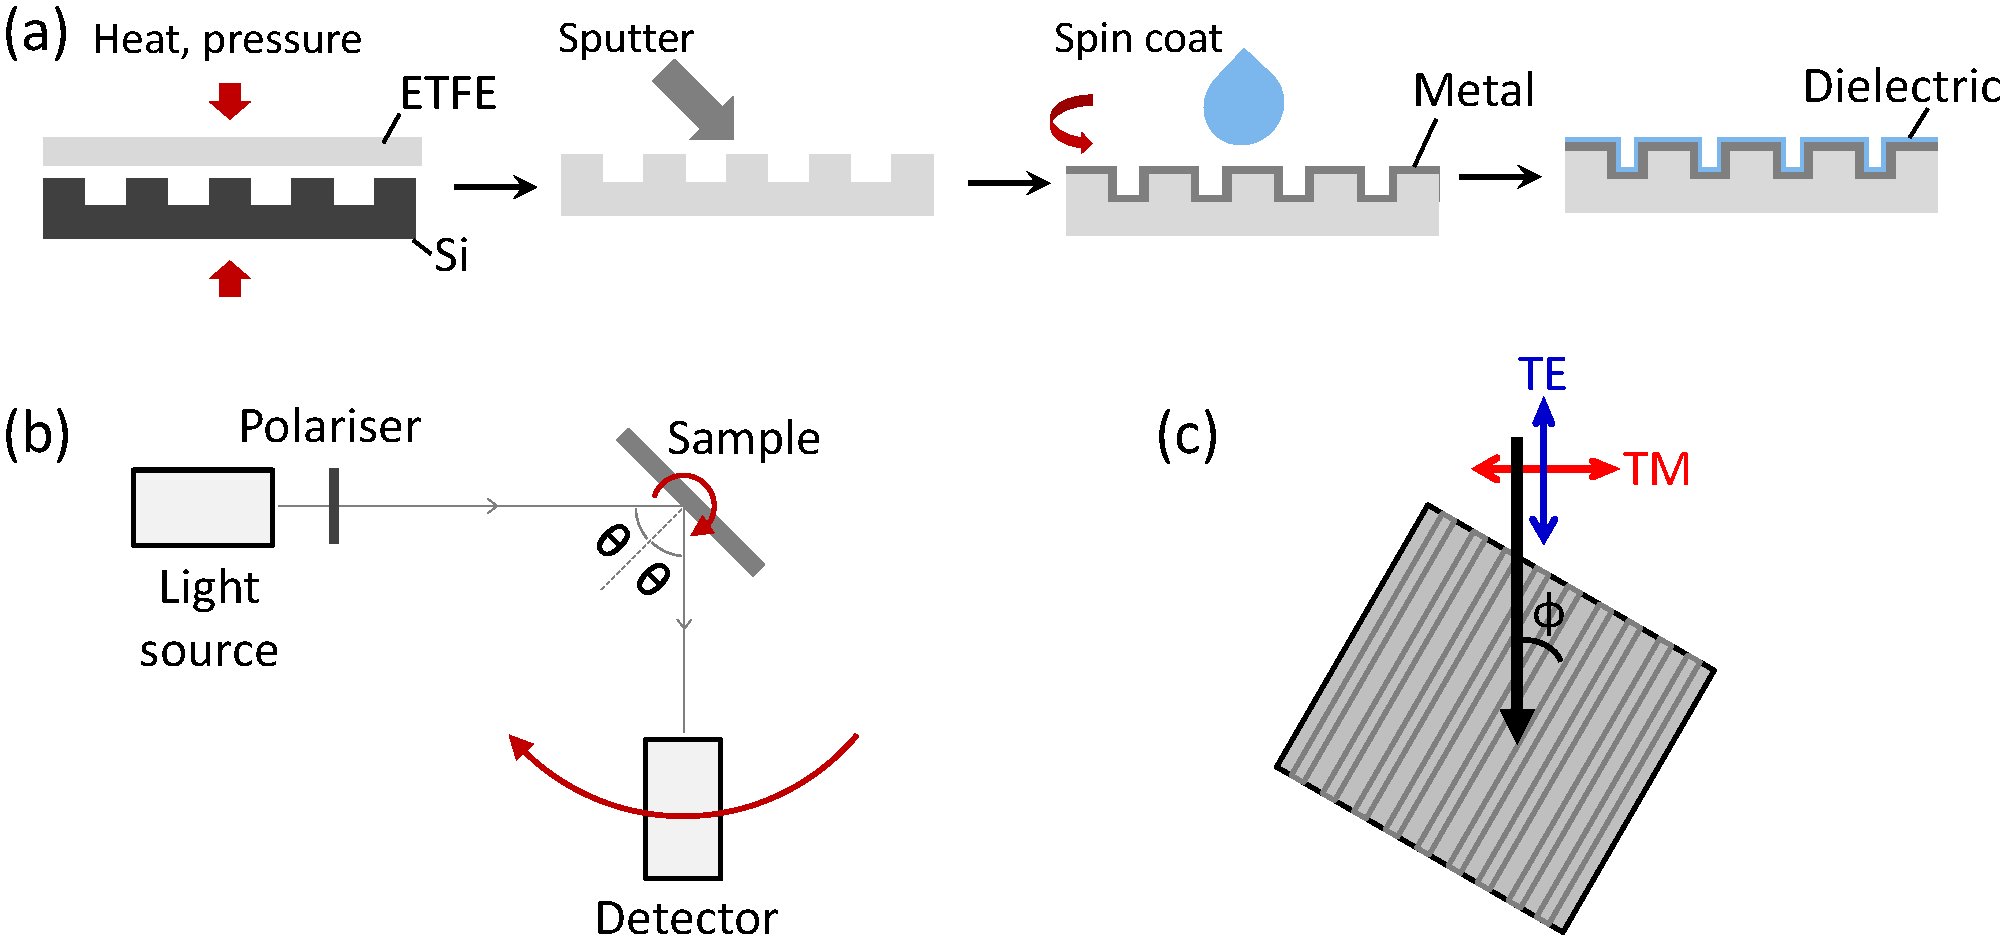
\includegraphics[width=\textwidth]{Fig1}
\caption{(a) Schematic of dielectric-coated metal grating fabrication. (b) Schematic of angle-dependent reflectivity measurement setup. (c) Relationship between the polarisation of incoming light and azimuthal angle $\phi$.}
\label{7Fig1}
\end{figure}
A schematic of the fabrication of dielectric-coated metal gratings is shown in Fig.\,\ref{7Fig1}(a). Gratings are fabricated in ethylene tetrafluoroethylene (ETFE) from nanopatterned silicon stamps using nanoimprinting. A sheet of ETFE (thickness 0.8\,mm) is placed on a silicon stamp, and heated to a temperature of $200^{\circ}$C before applying a pressure of 30\,Bar for 300s. The ETFE is then cooled to $90^{\circ}$ while maintaining the same pressure, before release from the stamps. An optically opaque metal layer ($\sim$120\,nm thick Ti/Ag) is deposited onto the polymer to form metal gratings. Chemically synthesised CHPI powder is dissolved in tetrahydrofuran and spin coated onto the gratings in a dehydrated atmosphere to produce a conformal coating. For PS-coated gratings, $M_w=500000$ PS powder is dissolved in toluene and spin coated onto the gratings. All samples are kept under a nitrogen atmosphere to prevent oxidation. Measurements by SEM and AFM of the metal and dielectric-coated gratings are used to extract the dimensions of the nanostructures. Specular reflection measurements are made as a function of the incident polar ($\theta$) and azimuthal ($\phi$) angles using a polarised broadband white light source ($215-2500$\,nm), with the geometry shown in Fig.\,\ref{7Fig1}(b,c). The sample properties are uniform over cm$^2$ areas, with small variations due to the depth and morphology of the coatings.

\section{Dielectric gratings}

\subsection{ETFE gratings}
AFM scans of the imprinted $D=417$\,nm ETFE grating structure [Fig.\,\ref{7Fig2}(a)] show the formation of a square-wave grating with depth 140\,nm and slit width 200\,nm [Fig.\,\ref{7Fig2}(b)]. TM and TE polarised reflectivity scans show $m=-1$ photonic modes according to Eq.[grating] (grey dashed lines on Figs.\,\ref{7Fig2}[c,e]), which appear as dips in the reflectivity [Figs.\,\ref{7Fig2}(d,f)]. In TE polarisation we also see the appearance of a redshifted photonic mode (grey dot-dashed line on Fig.\,\ref{7Fig2}(e)), corresponding to $n=1.4$ in Eq.[grating]. This fits well with the ETFE refractive index reported \cite{French2011}, thus attribute this redshifted mode to light which has penetrated the transmissive ETFE. For both polarisations the grating modes are no longer visible for $\phi>60^{\circ}$. Note also a dip in the reflectivity of TM scans at $\theta\approx50^{\circ}$ due to the Brewster angle of ETFE.
\begin{figure}[ht] 
\centering    
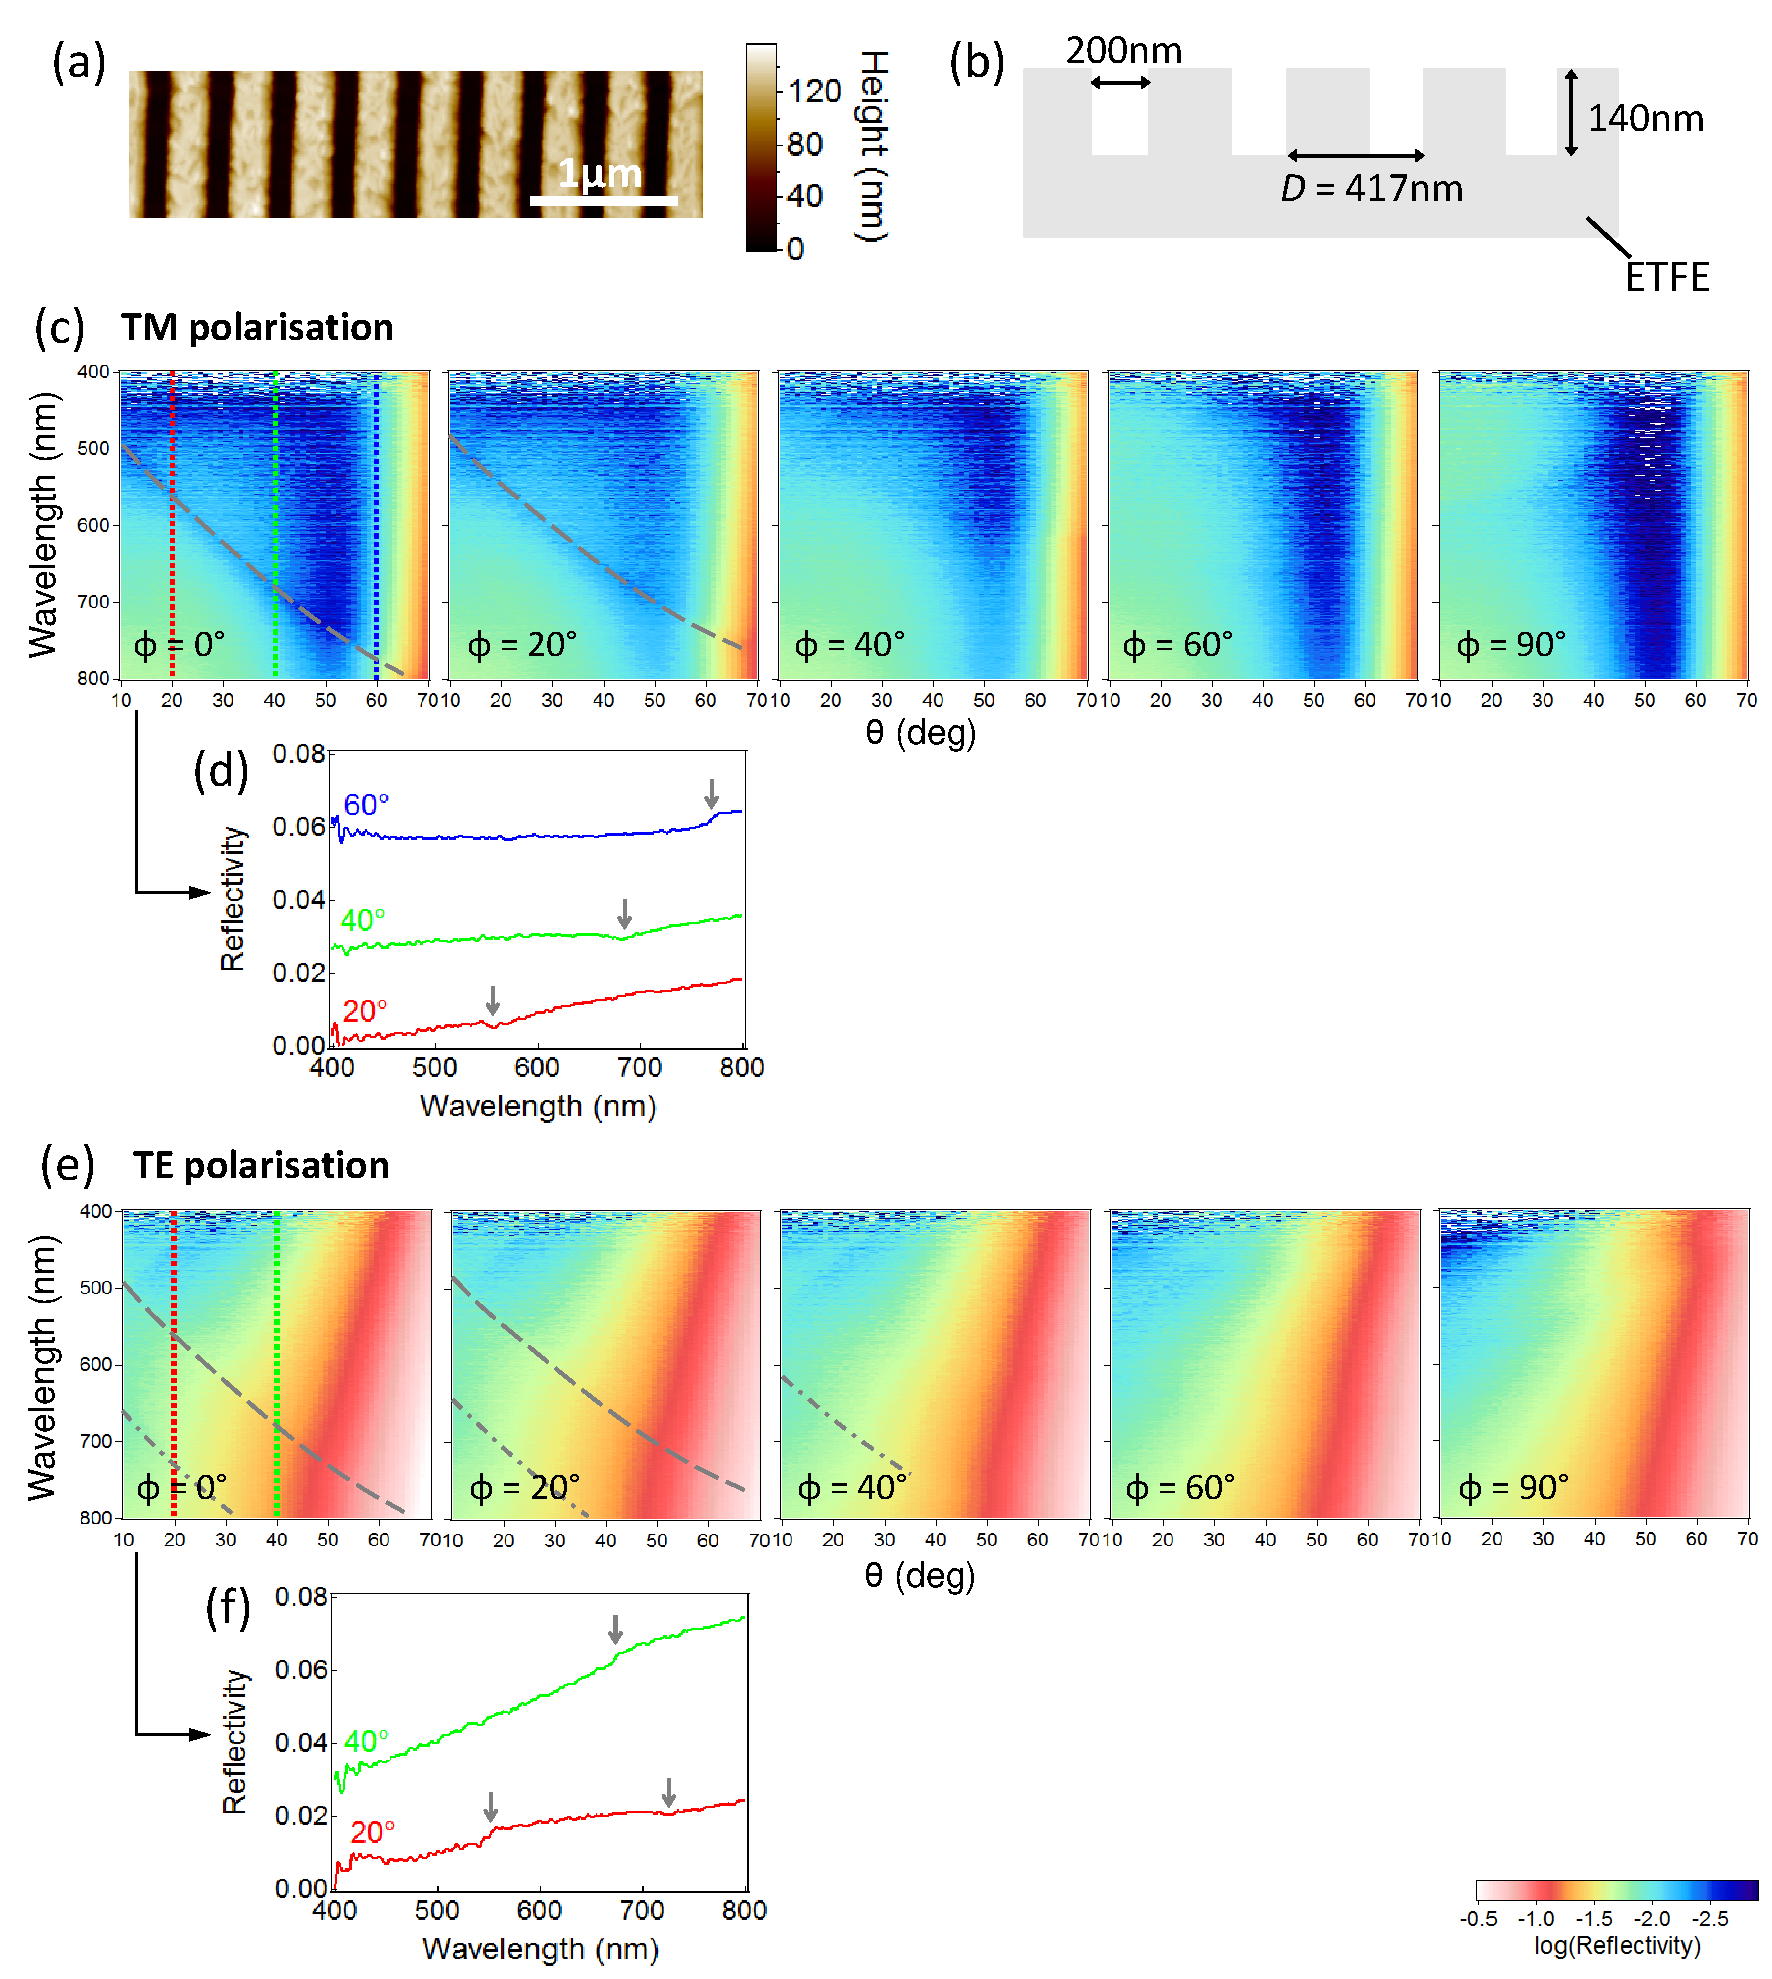
\includegraphics[width=\textwidth]{Fig2}
\caption{(a) AFM image and (b) schematic of ETFE grating structure. (c) TM polarised reflectivity scans of $D=417$\,nm ETFE grating at labelled $\phi$, and (d) reflectivity spectra at indicated $\theta$ values for $\phi=0^{\circ}$. (e,f) Same as above for TE polarisation. Photonic grating modes are indicated by grey lines/arrows on reflectivity scans/spectra respectively.}
\label{7Fig2}
\end{figure}

\subsection{CHPI-coated ETFE gratings}
The exciton resonance at 505\,nm dominates both the TM and TE reflectivity scans of CHPI-coated $D=417$\,nm ETFE gratings [Figs.\,\ref{7Fig3}(a,c)]. Diffractive photonic grating modes are also visible (marked by grey dot-dashed lines), and appear as Fano resonances in reflectivity due to interaction with the broad reflectivity background of the CHPI film [Figs.\,\ref{7Fig3}(b,d)]. The modes correspond $m=\pm1$ photonic modes are at the same positions as the $n=1.4$ redshifted modes in Fig.\,\ref{7Fig2}(e) and are thus attributed to the same source. In TM polarisation the diffractive modes are strongest for $\phi=90^{\circ}$, while for TE they are strongest at $\phi=0^{\circ}$. [Reason?] The Brewster angle in TM scans has changed to $\theta\approx62^{\circ}$ due to the larger refractive index of CHPI. Most notably, the grating modes do not interact with the excitons, even when crossings occur.
\begin{figure}[ht] 
\centering    
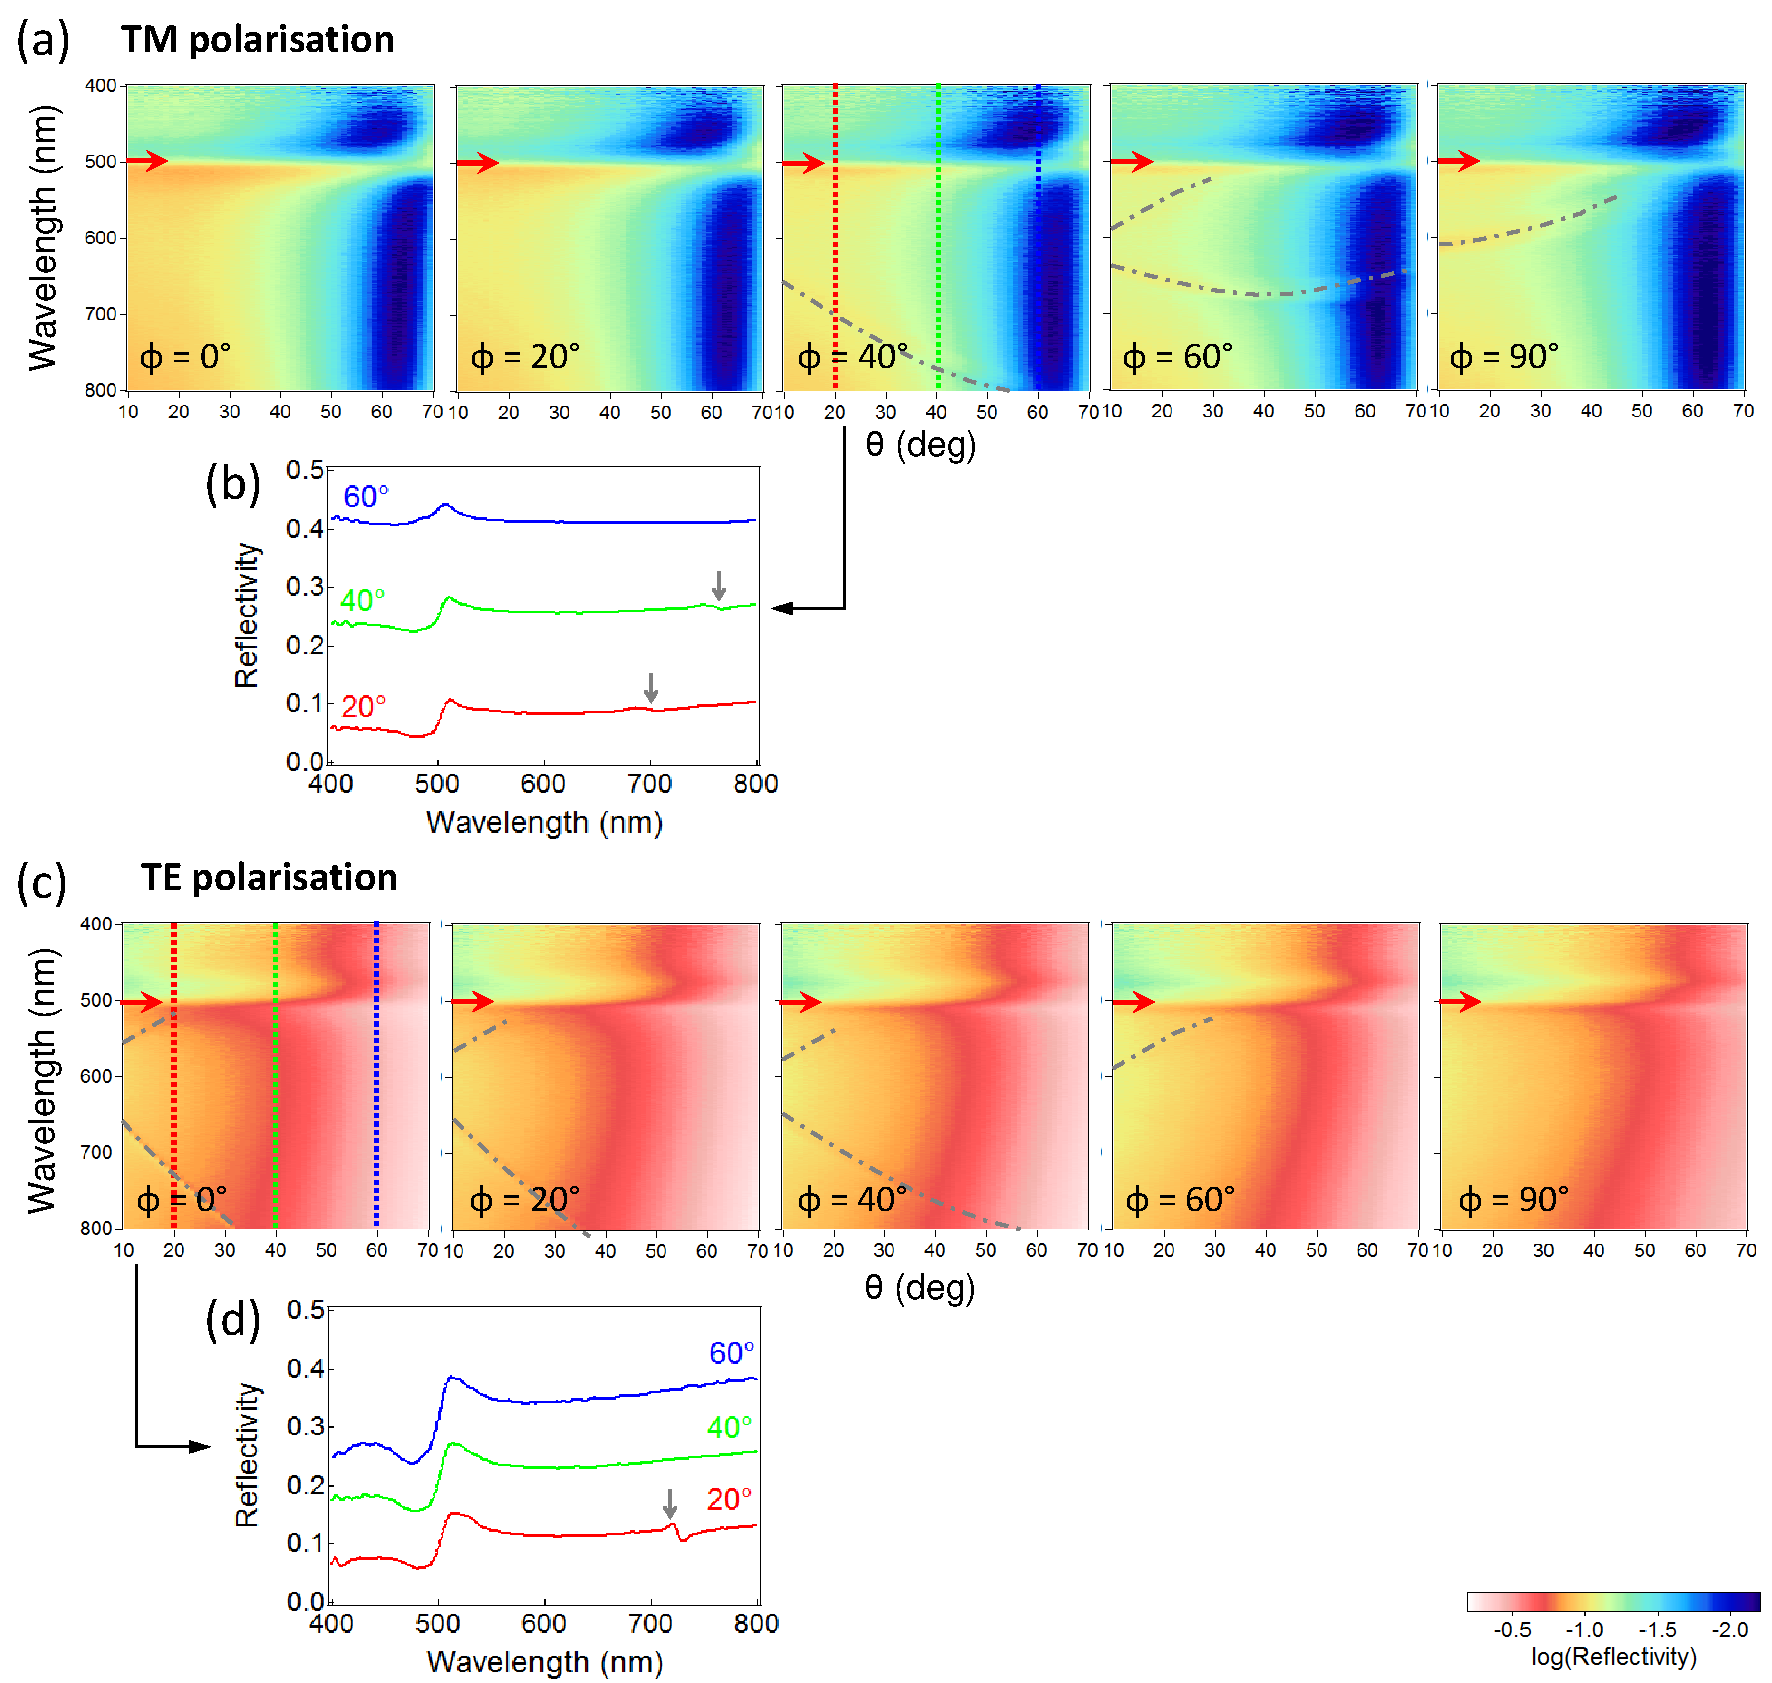
\includegraphics[width=\textwidth]{Fig3}
\caption{(a) TM polarised reflectivity scans of $D=417$\,nm CHPI-coated ETFE grating at labelled $\phi$, and (b) reflectivity spectra at indicated $\theta$ values for $\phi=0^{\circ}$. (c,d) Same as above for TE polarisation. Photonic grating modes are indicated by grey lines/arrows on reflectivity scans/spectra respectively, and excitons by red arrows.}
\label{7Fig3}
\end{figure}

\section{Non-plasmonic gratings}

\subsection{Ti gratings}
SEM image of the $D=417$\,nm Ti grating shows the roughness of the sputtered Ti film [Fig.\,\ref{7Fig4}(a)], while AFM measurements reveal a the formation of a more trapezoid grating profile, likely due to the initial imprinted EFTE grating rather than the sputtering process. Heat from the sputtering process also appeared to change the grating periodicity $D$ due to shrinking of ETFE, as the photonic grating modes in reflectivity scans [Figs.\,\ref{7Fig4}(c,e)] are best fit to $D=410$\,nm in Eq.[Grating]. Aside from the change in geometry, the appearance of $m=-1$ grating modes are very similar to the spectra of ETFE gratings, with modes appearing as dips in the reflectivity spectra. However the coupling to outgoing light is much weaker in TE polarisation, as shown by the comparative sizes of the dips in Figs.\,\ref{7Fig4}(d,f).
\begin{figure}[ht] 
\centering    
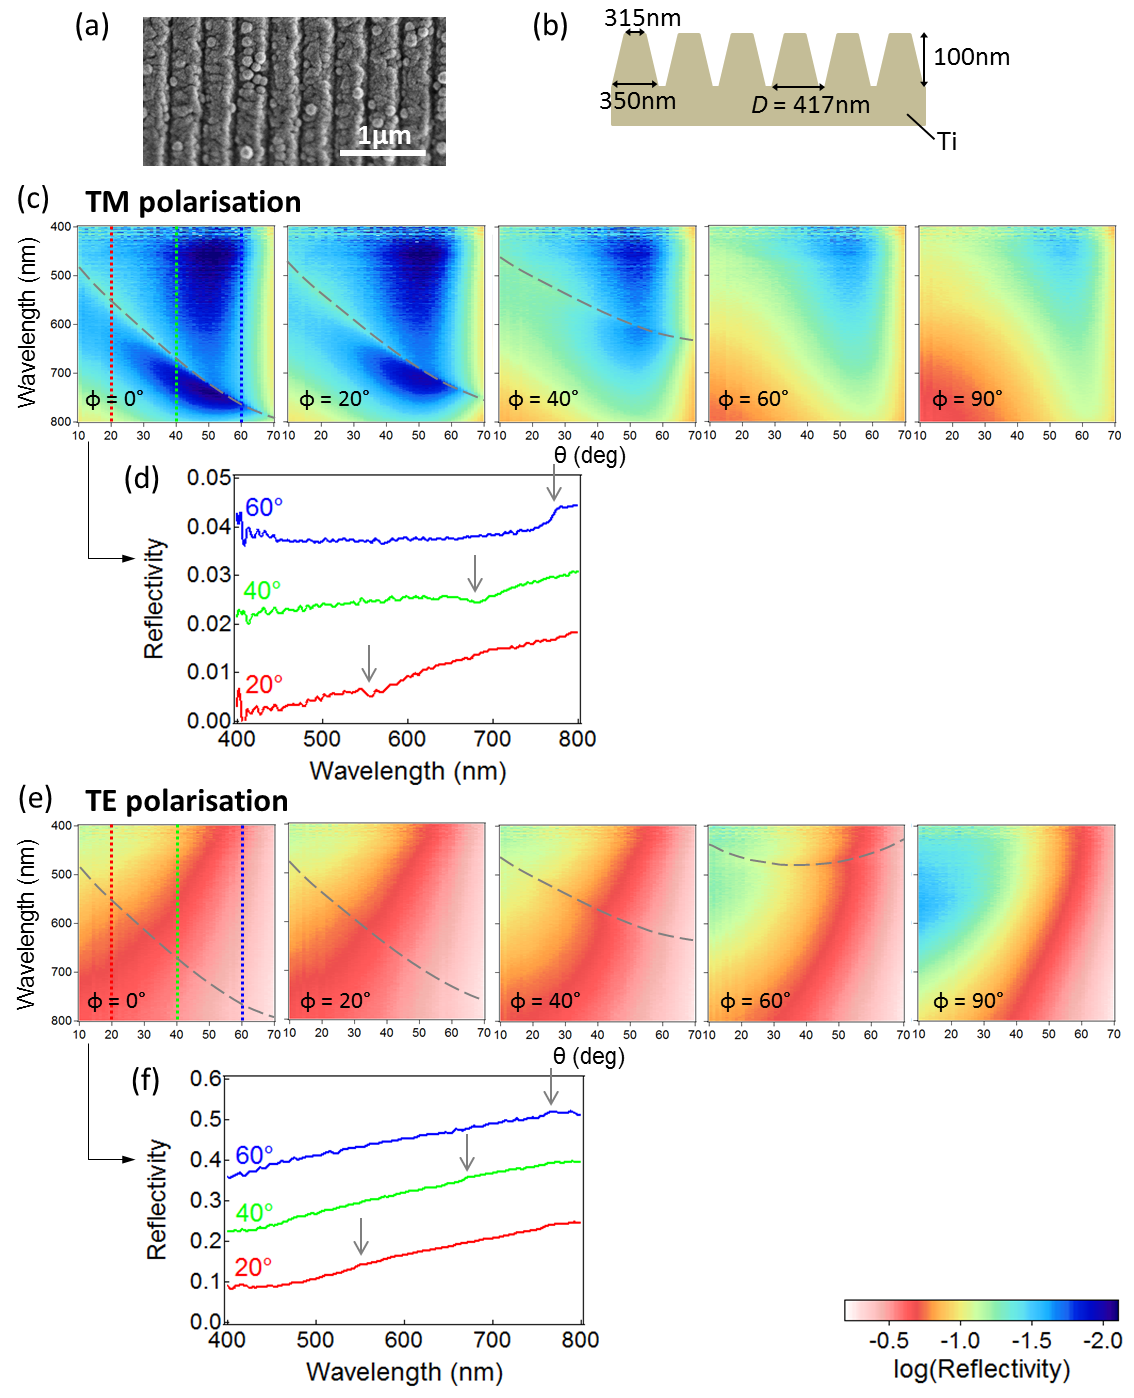
\includegraphics[width=\textwidth]{Fig4}
\caption{(a) SEM image and (b) schematic of Ti grating structure. (c) TM polarised reflectivity scans of $D=417$\,nm Ti grating at labelled $\phi$, and (d) reflectivity spectra at indicated $\theta$ values for $\phi=0^{\circ}$. (e,f) Same as above for TE polarisation. Photonic grating modes are indicated by grey lines/arrows on reflectivity scans/spectra respectively.}
\label{7Fig4}
\end{figure}

\subsection{CHPI-coated Ti gratings}
Polarised reflectivity spectra of CHPI-coated planar Ti film [Fig.\,\ref{7Fig5}] shows the appearance of an exciton resonance at 505\,nm, showing that the excitons are unaffected by the metal film below. The experimental data fits well to transfer matrix simulations of 70\,nm CHPI-coated 120\,nm Ti film, and the differences observed can be attributed to non-uniformity and roughness in both the CHPI and Ti films.
\begin{figure}[ht] 
\centering    
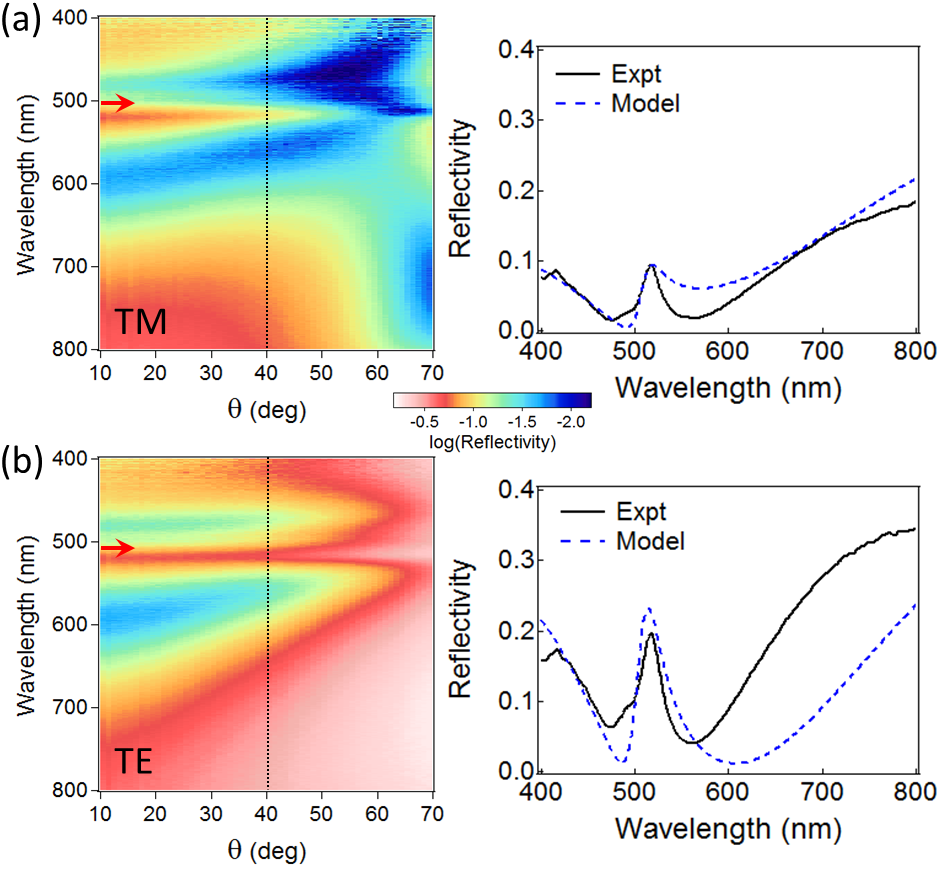
\includegraphics[width=0.6\textwidth]{Fig5}
\caption{Specular reflectivity scans of 70\,nm CHPI film on 120\,nm planar Ti film with (a) TM and (b) TE polarised light. Excitons are marked by red arrows. Spectra at $\theta=40^{\circ}$ are plotted with those predicted by transfer matrix simulations (right).}
\label{7Fig5}
\end{figure}

\begin{figure}[ht] 
\centering    
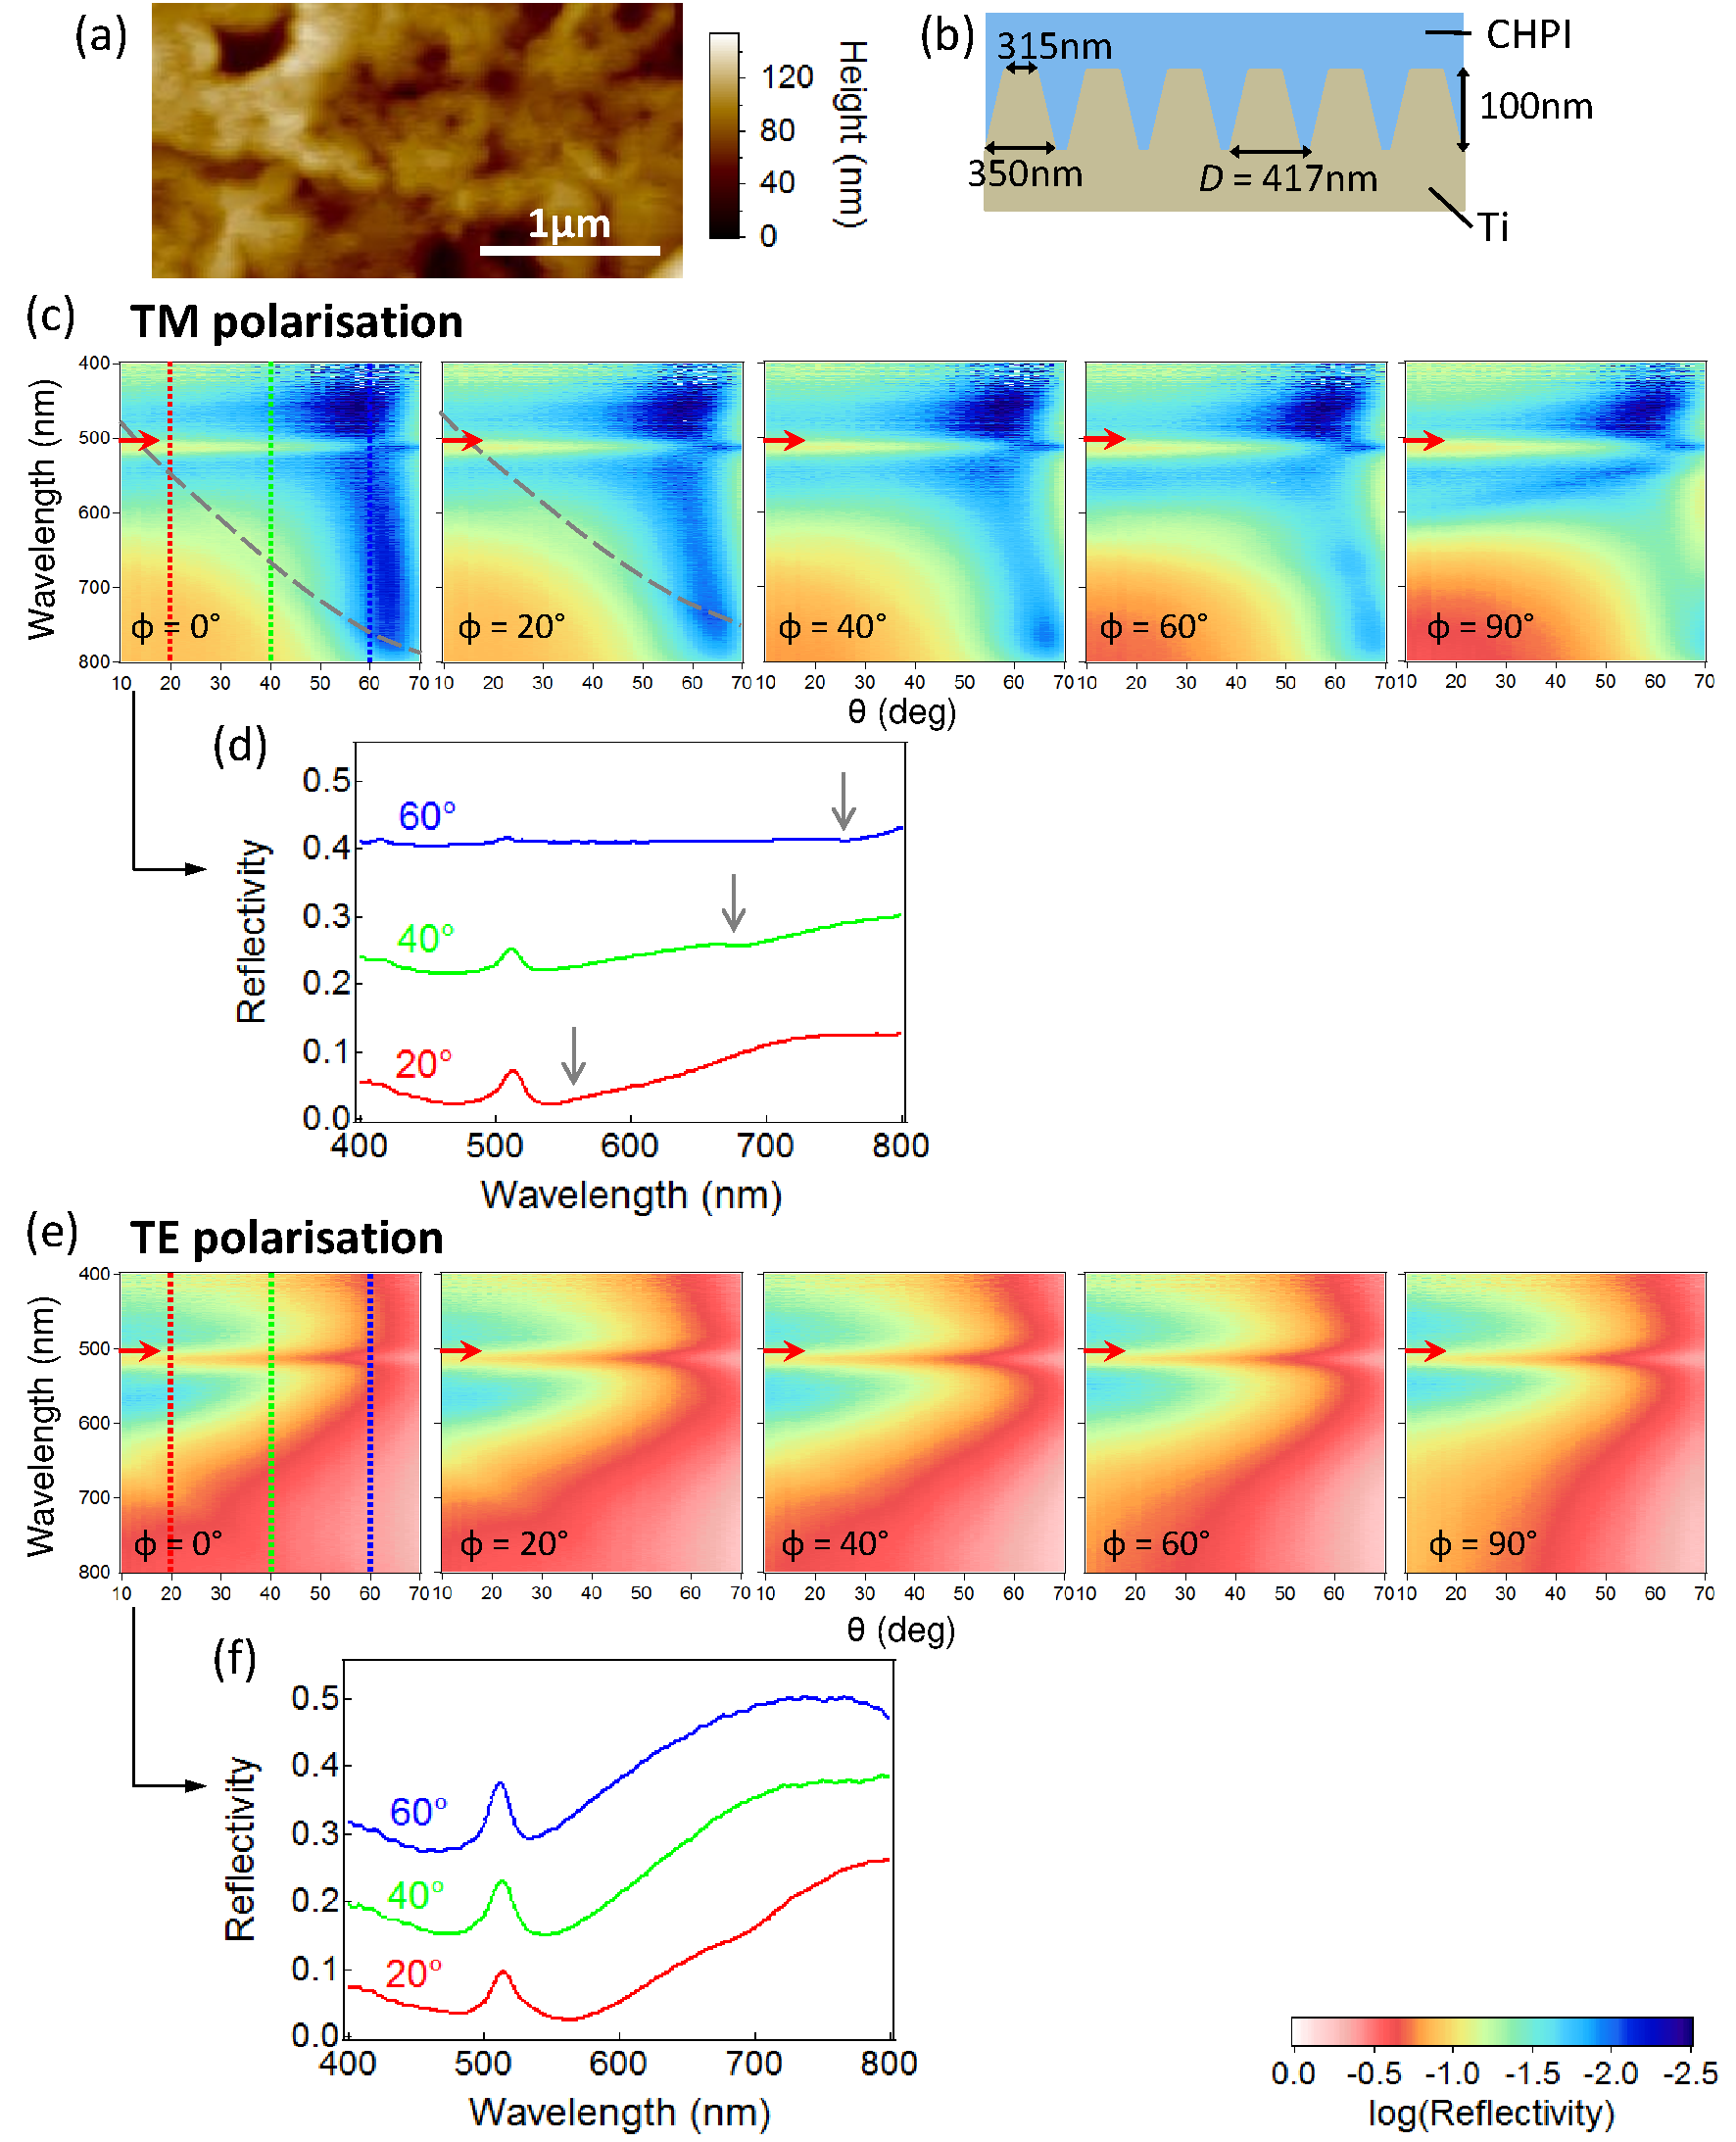
\includegraphics[width=\textwidth]{Fig6}
\caption{(a) AFM image and (b) schematic of CHPI-coated Ti grating structure. (c) TM polarised reflectivity scans of $D=417$\,nm CHPI-coated Ti grating at labelled $\phi$, and (d) reflectivity spectra at indicated $\theta$ values for $\phi=0^{\circ}$. (e,f) Same as above for TE polarisation. Photonic grating modes are indicated by grey lines/arrows on reflectivity scans/spectra respectively, and excitons by red arrows.}
\label{7Fig6}
\end{figure}
AFM measurements of CHPI-coated $D=417$\,nm Ti grating show no appearance of the grating structure [Fig.\,\ref{7Fig6}(a)], and from this we conclude that the grating structure has been completely immersed in the non-uniform CHPI film [Fig.\,\ref{7Fig6}(b)]. As with CHPI-coated ETFE gratings, the exciton resonance at 505\,nm dominates reflectivity spectra for both TM and TE polarisation [Figs.\,\ref{7Fig6}(c,e)]. Although very weak dips can be seen in reflectivity to indicate diffractive $m=-1$ grating modes in TM polarisation [Fig.\,\ref{7Fig6}(d)], coupling of TE-polarised light to grating modes is so weak that spectra look essentially like that of the CHPI-coated planar Ti film [Fig.\,\ref{7Fig6}(f)]. In both cases there are no interactions between CHPI excitons and modes of the Ti grating.

\section{Plasmonic gratings}

\subsection{Ag gratings}
Fig.\,\ref{7Fig7} shows reflectivity scans for Ag gratings with periodicities $D=556, 417, 278$\,nm. The spectra for all three gratings show the same features: in TM polarisation a sharp threshold anomaly is observed, whose dispersion follows Eq.[grating] for the $m=\pm1$ modes (grey dashed lines). A redshifted dip follows for the resonance anomaly, indicating the presence of excited SPPs (black dashed lines). In TE polarisation we don't observe any anomaly features due to the inability to excite SPPs, instead we see the $m=\pm1$ photonic modes.
\begin{figure}[ht] 
\centering    
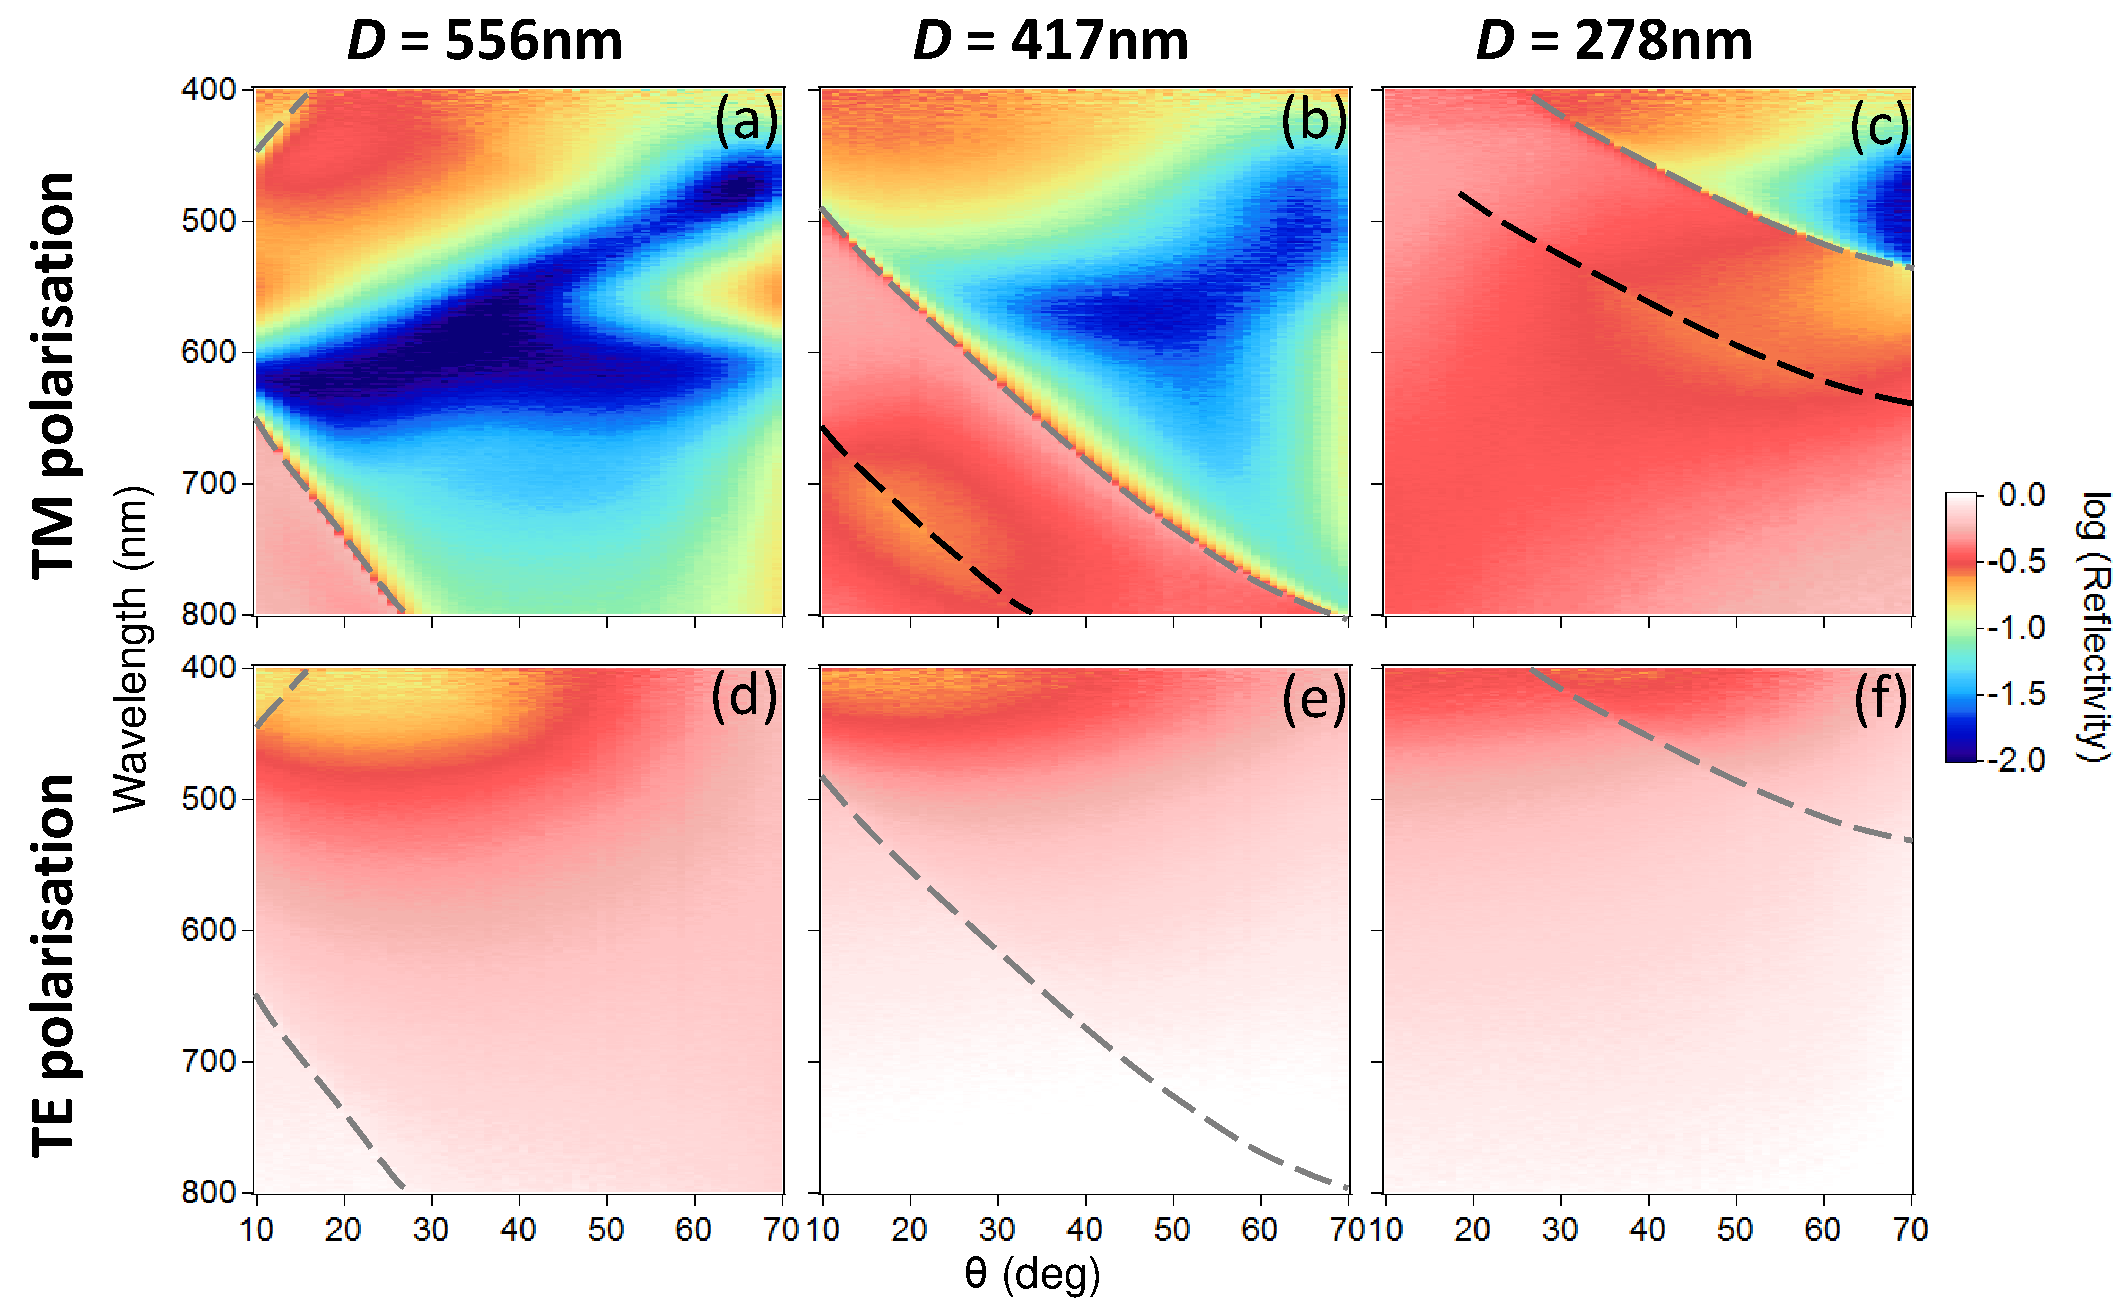
\includegraphics[width=0.8\textwidth]{Fig7}
\caption{Specular reflectivity scans of uncoated Ag gratings with the labelled periodicity $D$ and polarisation of light. Photonic grating modes (threshold anomalies) are marked by grey dashed lines, and plasmonic grating modes (resonance anomalies) are maked by black dashed lines.}
\label{7Fig7}
\end{figure}

Concentrating on the $D=417$\,nm grating, we see that the sputtered Ag also shows some roughness [Fig.\,\ref{7Fig8}(a)], and AFM measurements indicate a square-wave grating with depth 140\,nm and slit width 130\,nm [Fig.\,\ref{7Fig8}(b)]. In reflectivity [Fig.\,\ref{7Fig8}(c,e)] the threshold (grey dashed lines) and resonance (black dashed lines) anomalies shift as expected from Eq.[grating] with $\phi$ in TM polarisation, and appear as the expected sharp change in intensity/dip in spectra [Fig.\,\ref{7Fig8}(d)]. The resonance anomaly becomes weaker with increasing $\phi$ and is no longer observed at $\phi=60^{\circ}$ as it becomes harder to couple to SPPs in this polarisation. For this same reason no anomalies are observed in TE polarisation at low $\phi$, where the photonic modes appear as rather weak peaks in the spectra [Fig.\,\ref{7Fig8}(f)]. We would expect to observe anomalies at $\phi=90^{\circ}$ in TE polarisation, however the energy of the mode is too high for our measurement range here. The broad dip seen at $\phi=60^{\circ}$ in both polarisations and $\phi=90^{\circ}$ in TE polarisation is assigned to a Fabry-Perot interference mode of light reflected from the top and bottom surfaces of the grating. The mode doesn't change in position with $\phi$ as expected, and extrapolates to $\sim600$\,nm at $\theta=0^{\circ}$, which fits the height of the gratings as seen in AFM measurements.
\begin{figure}[ht] 
\centering    
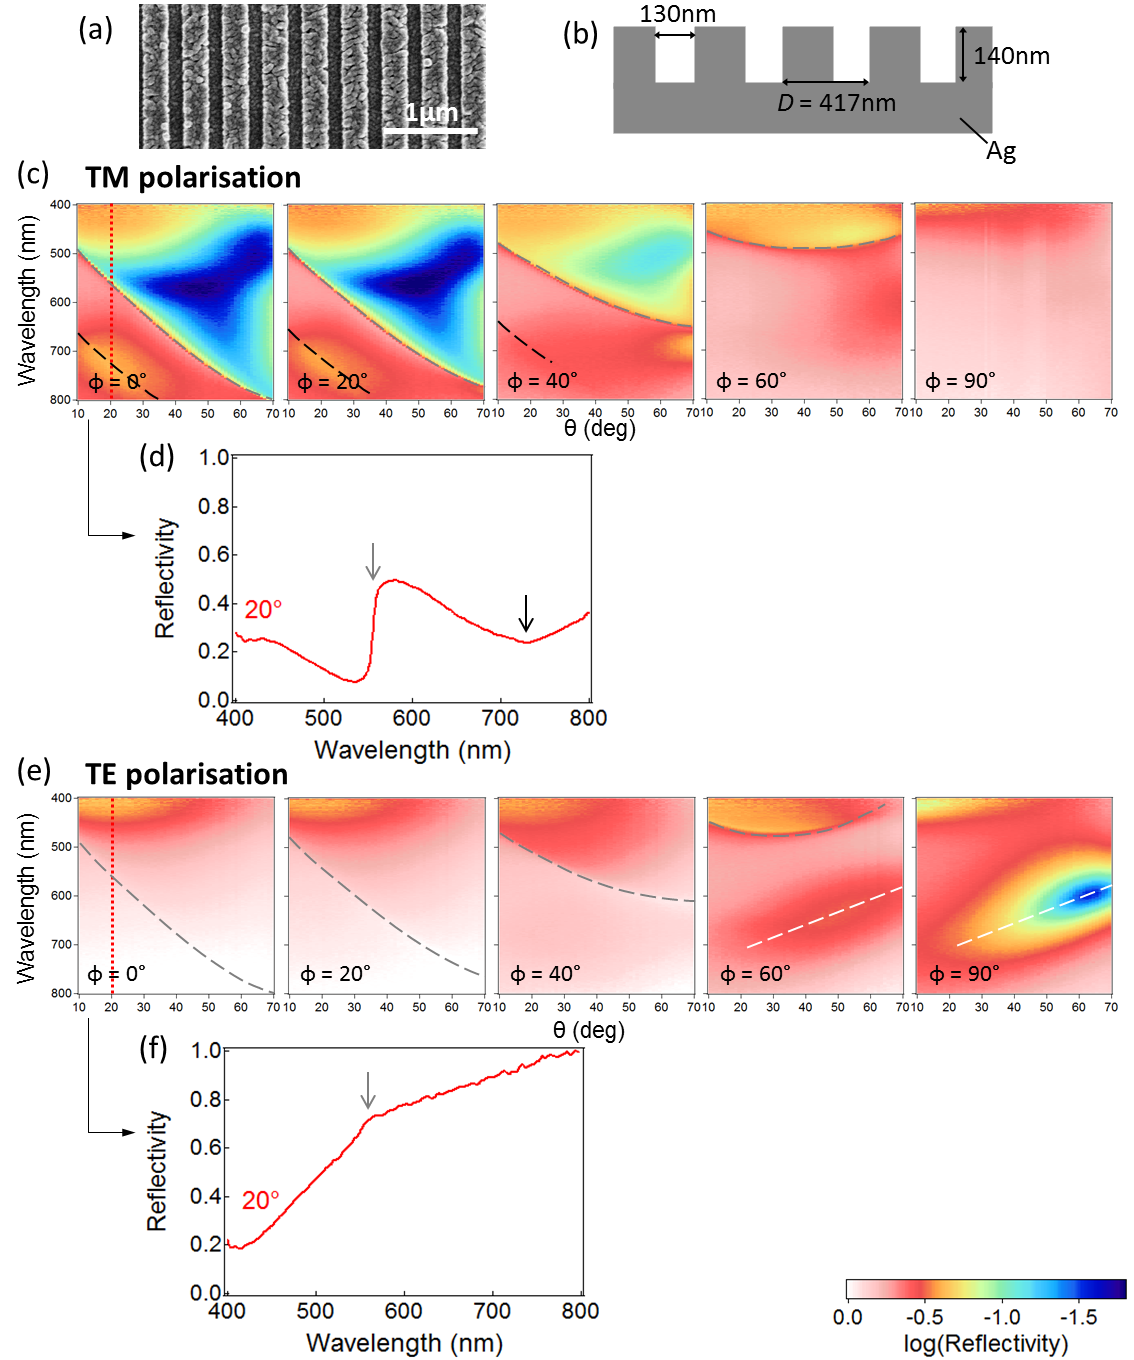
\includegraphics[width=\textwidth]{Fig8}
\caption{(a) SEM image and (b) schematic of Ag grating structure. (c) TM polarised reflectivity scans of $D=417$\,nm Ag grating at labelled $\phi$, and (d) reflectivity spectra at indicated $\theta$ values for $\phi=0^{\circ}$. (e,f) Same as above for TE polarisation. Photonic grating modes (threshold anomalies) are indicated by grey lines/arrows on reflectivity scans/spectra respectively, and plasmonic gratings modes (resonance anomalies) by black lines/arrows.}
\label{7Fig8}
\end{figure}

We use finite element method (FEM) to model the electromagnetic nearfield of the grating modes to understand their behaviour. The modelled spectra for $\phi=0^{\circ} \lambda=600$\,nm agrees very well with the features of the experimental data [Fig.\,\ref{7Fig9}(a)], but has a larger reflectivity overall due to roughness on the experimentally created Ag gratings. The low reflectivity region at high $\theta$ is caused by low efficiency of the specularly reflected order. Instead the strongest coupling is to the $-1$ diffracted order, as evidenced by the wavefronts of $E$-field intensity in a diagonal direction in Fig.\,\ref{7Fig9}(b). The modelled $H_z$ field component for $\theta=30^{\circ} \lambda=700$\,nm shows at various points in the optical cycle [Fig.\,\ref{7Fig9}(c)] shows that the resonance anomaly does indeed behave like SPP on the surface of the metal, in this case travelling towards the left of the grating. 
\begin{figure}[ht] 
\centering    
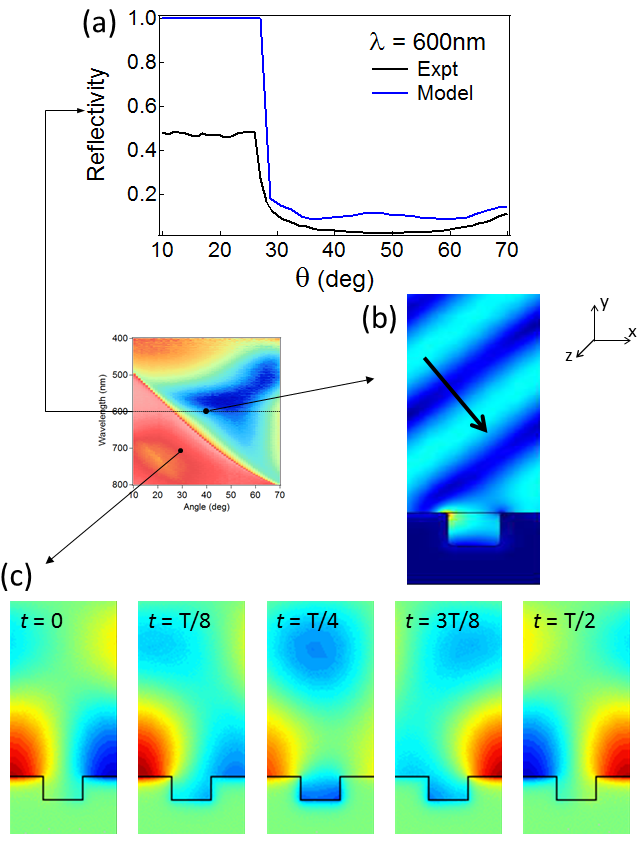
\includegraphics[width=0.8\textwidth]{Fig9}
\caption{(a) Experimental and modelled TM reflectivity spectra for $\phi=0^{\circ}$. (b) Time averaged $E$-field intensity ($\vec{E}\cdot\vec{E}$) profile for $\lamda=600$\,nm $\theta=40^{\circ}$. (c) $H_z$ nearfield profile at labelled points of the optical cycle for $\lambda=700$\,nm $\theta=30^{\circ}$.}
\label{7Fig9}
\end{figure}

The position of the threshold anomaly is fixed by the periodicity of the structure, however as the resonance anomaly is a Fano resonance due to the interference between diffracted light and SPPs we expect the position of this to depend much more sensitively on the geometry of the grating. Fig.\,\ref{7Fig10} shows the structures and TM reflectivity scans at $\phi=0^{\circ}$ for three difference gratings, ranging from a square-wave grating [Fig.\,\ref{7Fig10}(a)] to a more sinusiodal grating [Fig.\,\ref{7Fig10}(b,c)], and these geometric differences are caused by small changes in the nanoimprinting conditions. We see that the sharp threshold anomalies (grey dashed lines) remain in the same positions for all three gratings, barring small changes in the periodicity due to the shrinkage of ETFE. However the width and positions of the resonance anomaly dips vary greatly with geometry. As shown in the changing the grating geometry during modelling, square-wave gratings produce the widest resonance anomalies, and sinusoidal gratings the sharpest resonances. We also observe a dispersionless mode in the reflectivity at $\sim450$\,nm for the more sinusoidal gratings. This could be due to the presence of a channel plasmon, which requires a narrowing of the gap as seen in Fig.\,\ref{7Fig10}(c) in particular.
\begin{figure}[ht] 
\centering    
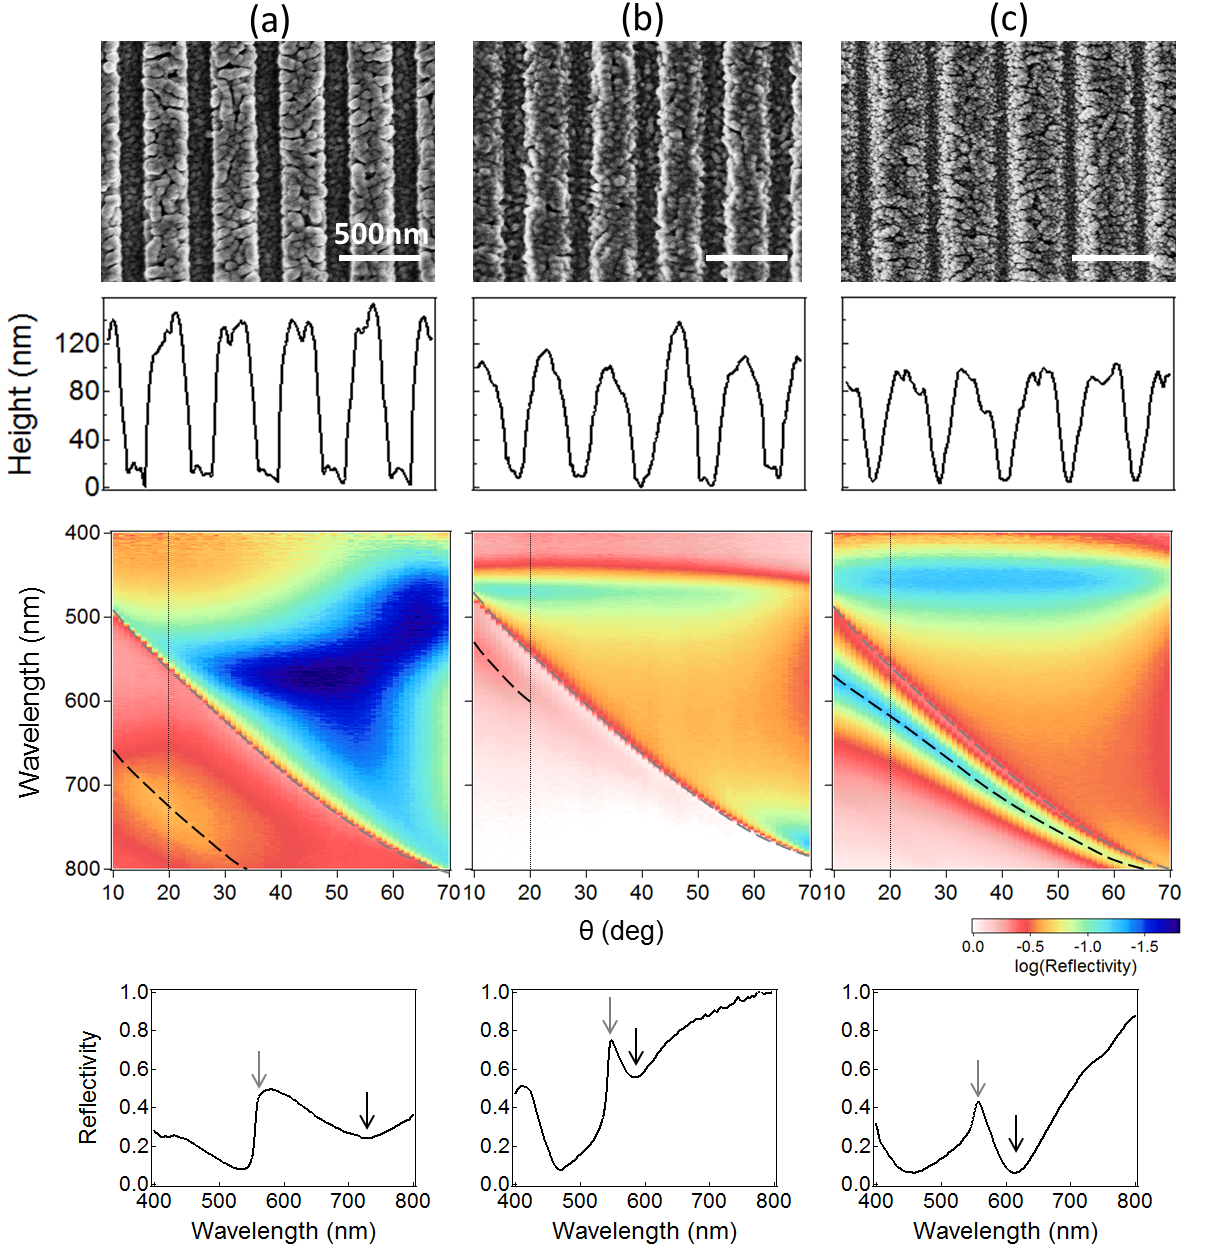
\includegraphics[width=\textwidth]{Fig10}
\caption{Effect of grating geometry on the optical spectra of $D=417$\,nm Ag gratings. (From top) SEM image, AFM profile, TM specular reflectivity scans at $\phi=0^{\circ}$, and reflectivity spectra at $\theta=20^{\circ}$ for three gratings. Photonic grating modes (threshold anomalies) are marked by grey dashed lines/arrows, and plasmonic grating modes (resonance anomalies) by black dashed lines/arrows on reflectivity scans/spectra respectively.}
\label{7Fig10}
\end{figure}

\subsection{PS-coated Ag gratings}
Fig.\,\ref{7Fig11}(a) shows the AFM image of a PS-coated Ag grating, where the grating structure is clearly observable, however only with an average height of 5\,nm. From this we deduce the the Ag grating is almost submerged beneath the non-uniform PS layer [Fig.\,\ref{7Fig11}(b)]. The presence of the PS overcoating increases the complexity of the reflectivity spectra by allowing more modes to be accessed. In TM polarisation, both photonic (grey dashed lines) and redshifted plasmonic modes (black dashed lines) can be observed [Fig.\,\ref{7Fig11}(c)]. Both of these modes are also observed in TE polarisation [Fig.\,\ref{7Fig11}9e)], although the photonic mode is much weaker. At high $\phi$ in TM polarisation, a potential second set of plasmonic modes can be seen (black dot-dashed lines), indicating two refractive index environments, perhaps the top and bottom surface of the grating where the PS coverages are different. We also see a broader mode at $\sim520$\,nm for $\phi=0^{\circ} \theta=10^{\circ}$, which redshifts slighly with increasing $\phi$ while maintaining a similar shape (purple dashed line). A similar mode can be observed in TE polarisation, although not at exactly the same position.
\begin{figure}[ht] 
\centering    
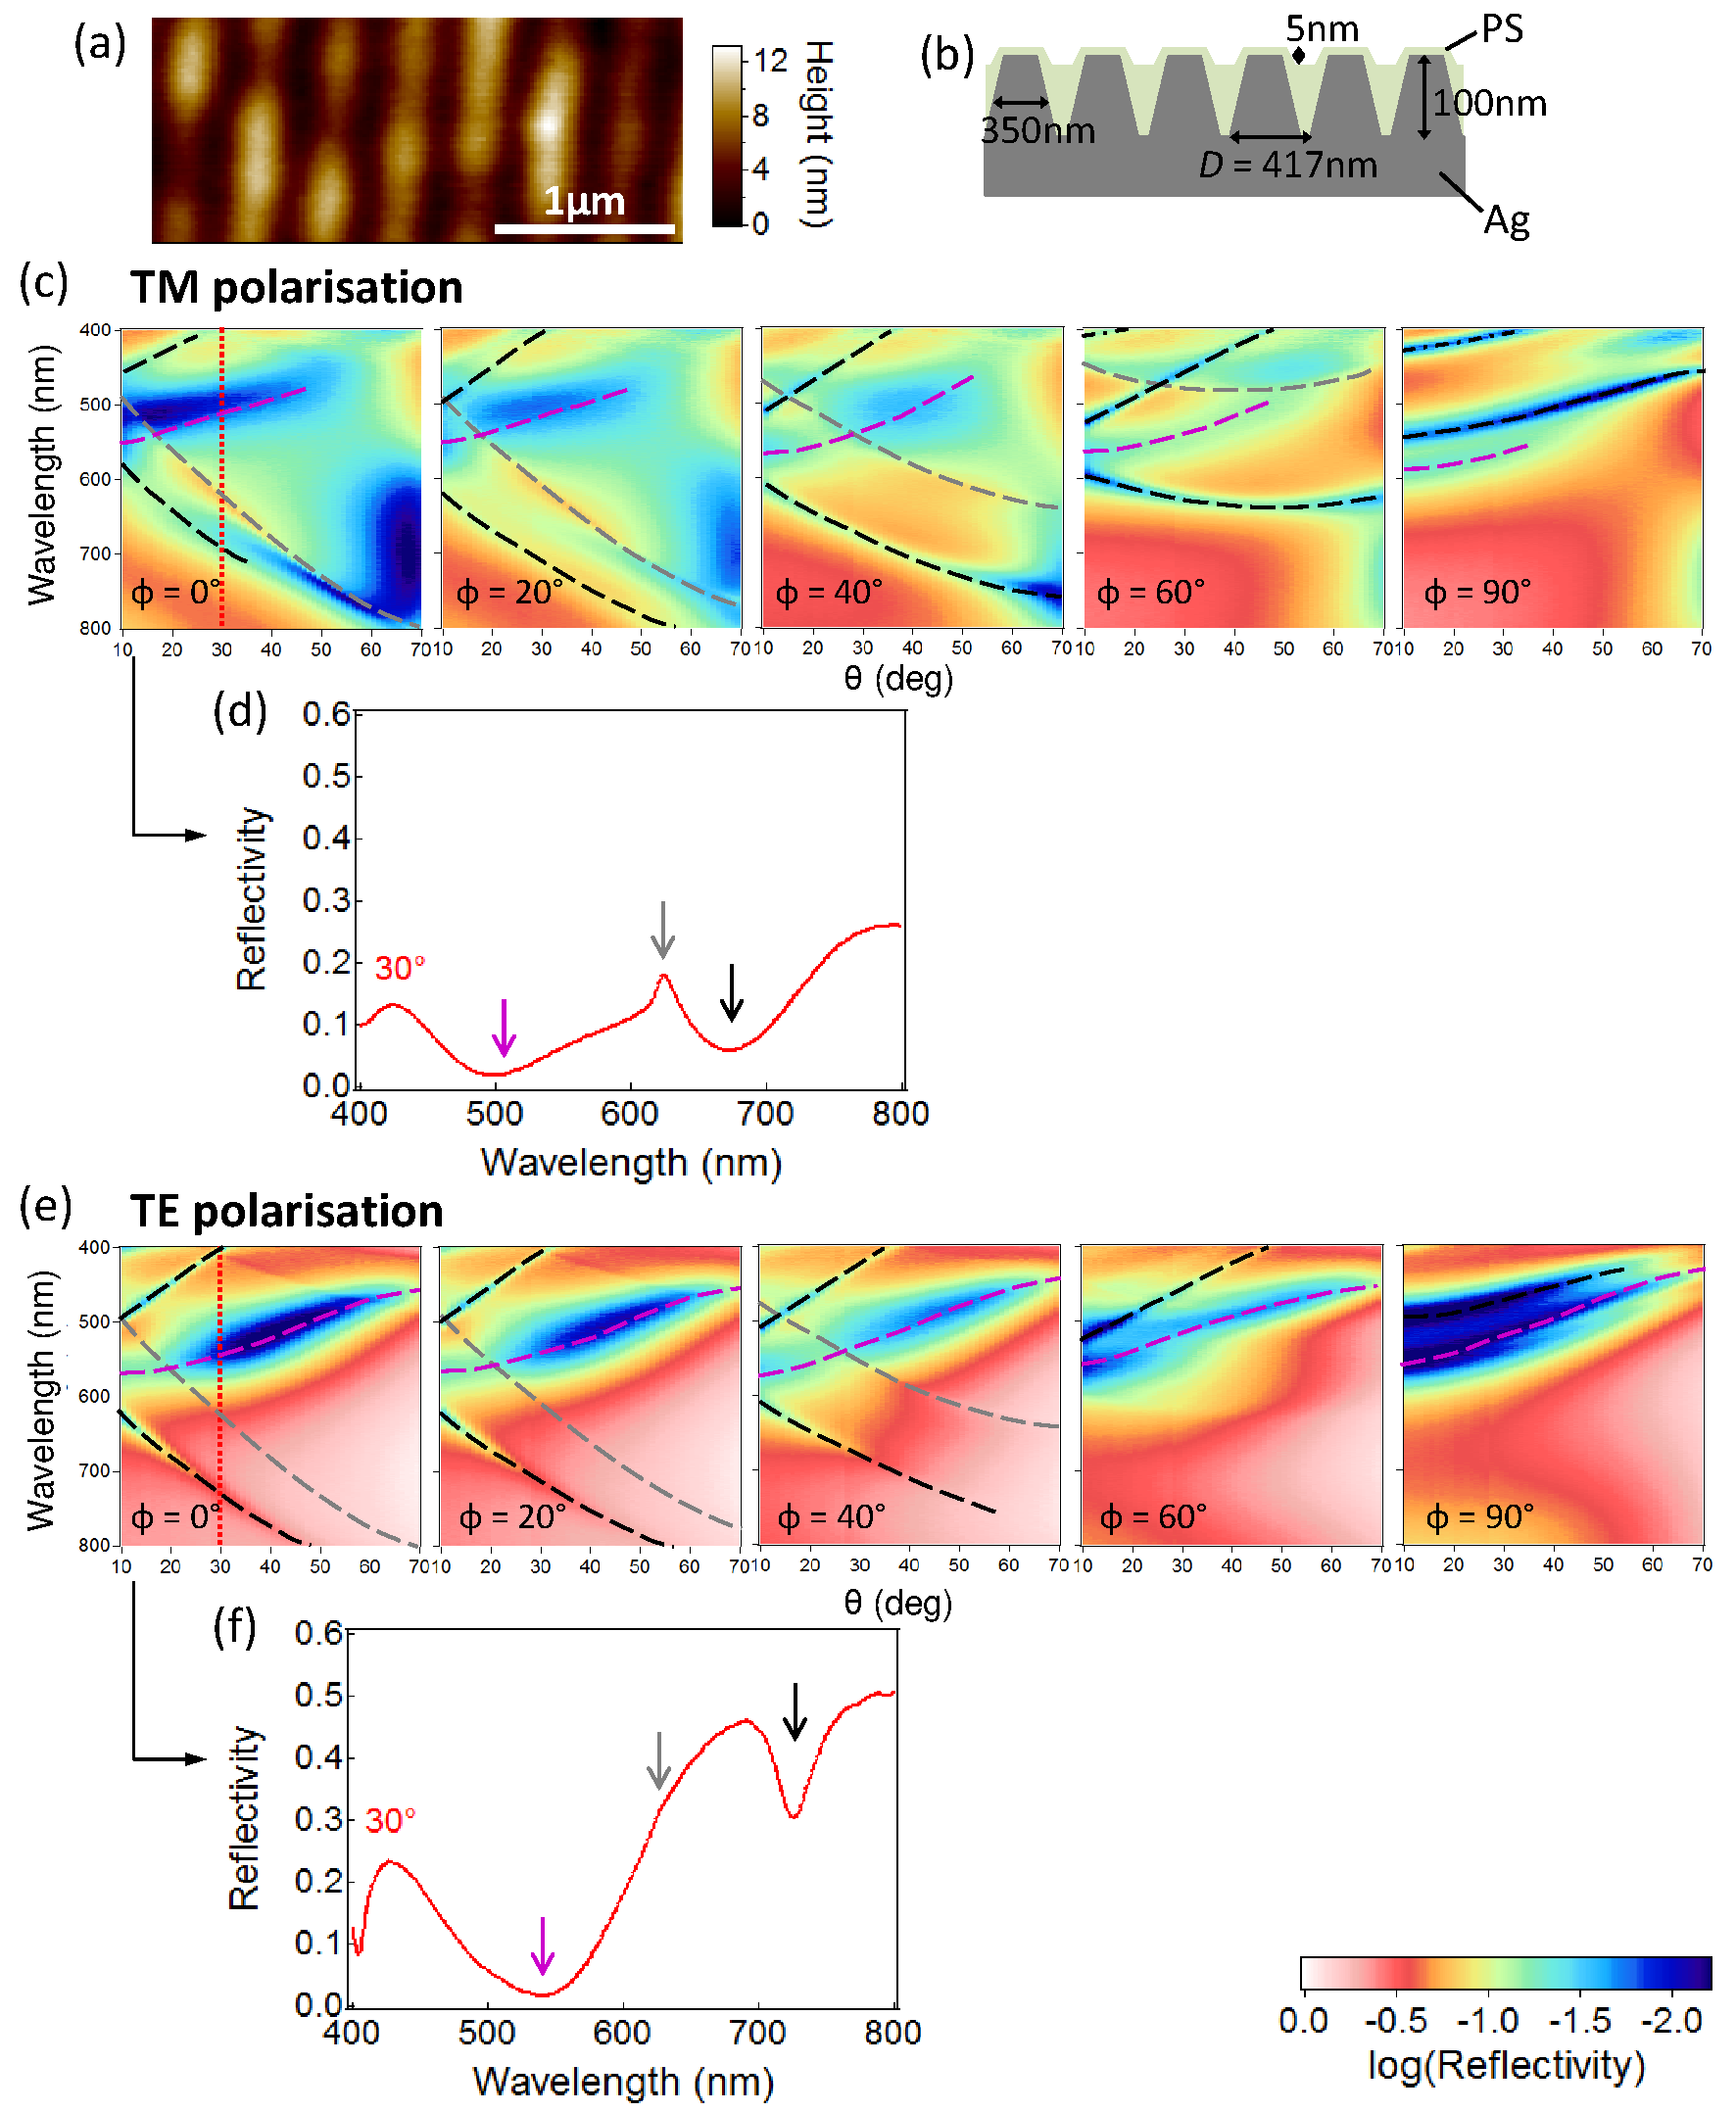
\includegraphics[width=\textwidth]{Fig11}
\caption{(a) AFM image and (b) schematic of PS-coated Ag grating structure. (c) TM polarised reflectivity scans of $D=417$\,nm PS-coated Ag grating at labelled $\phi$, and (d) reflectivity spectra at indicated $\theta$ value for $\phi=0^{\circ}$. (e,f) Same as above for TE polarisation. Photonic grating modes are indicated by grey lines/arrows on reflectivity scans/spectra respectively,plasmonic gratings modes by black lines/arrows, and waveguide modes by purple lines arrows.}
\label{7Fig11}
\end{figure}

Using FEM modelling, we observe two types of modes at $\phi=0^{\circ}$ at TM polarisation. A mode at higher energy has field intensity concentrated at the top surface of the grating, evanescently decaying from the Ag surface [Fig.\,\ref{7Fig12}(a)]. Taking snapshots throughout the optical cycle, the mode appears to be a quasiparticle travelling along the top surface of the grating as expected in the $\phi=90^{\circ}$ geometry [Fig.\,\ref{7Fig12}(b)]. By varying the geometry of the grating, we see that the mode decreases in energy as $D$ increases, increases in energy with the slit width, and is unaffected by grating height, thus showing the behaviour expected for an SPP mode. The field intensity of the lower energy mode is mainly concentrated in the slit of the grating [Fig.\,\ref{7Fig12}(c)], and again appears to travel along the slit throughout the optical cycle [Fig.\,\ref{7Fig12}(d)]. The energy of the mode is unaffected by $D$ or the grating height, and decreases as the slit width increases. This behaviour for a mode waveguided by the grating slit, and according to Eq.[waveguide] the dispersion fits that of a $\textnormal{TE}_{10}$ mode. 
\begin{figure}[ht] 
\centering    
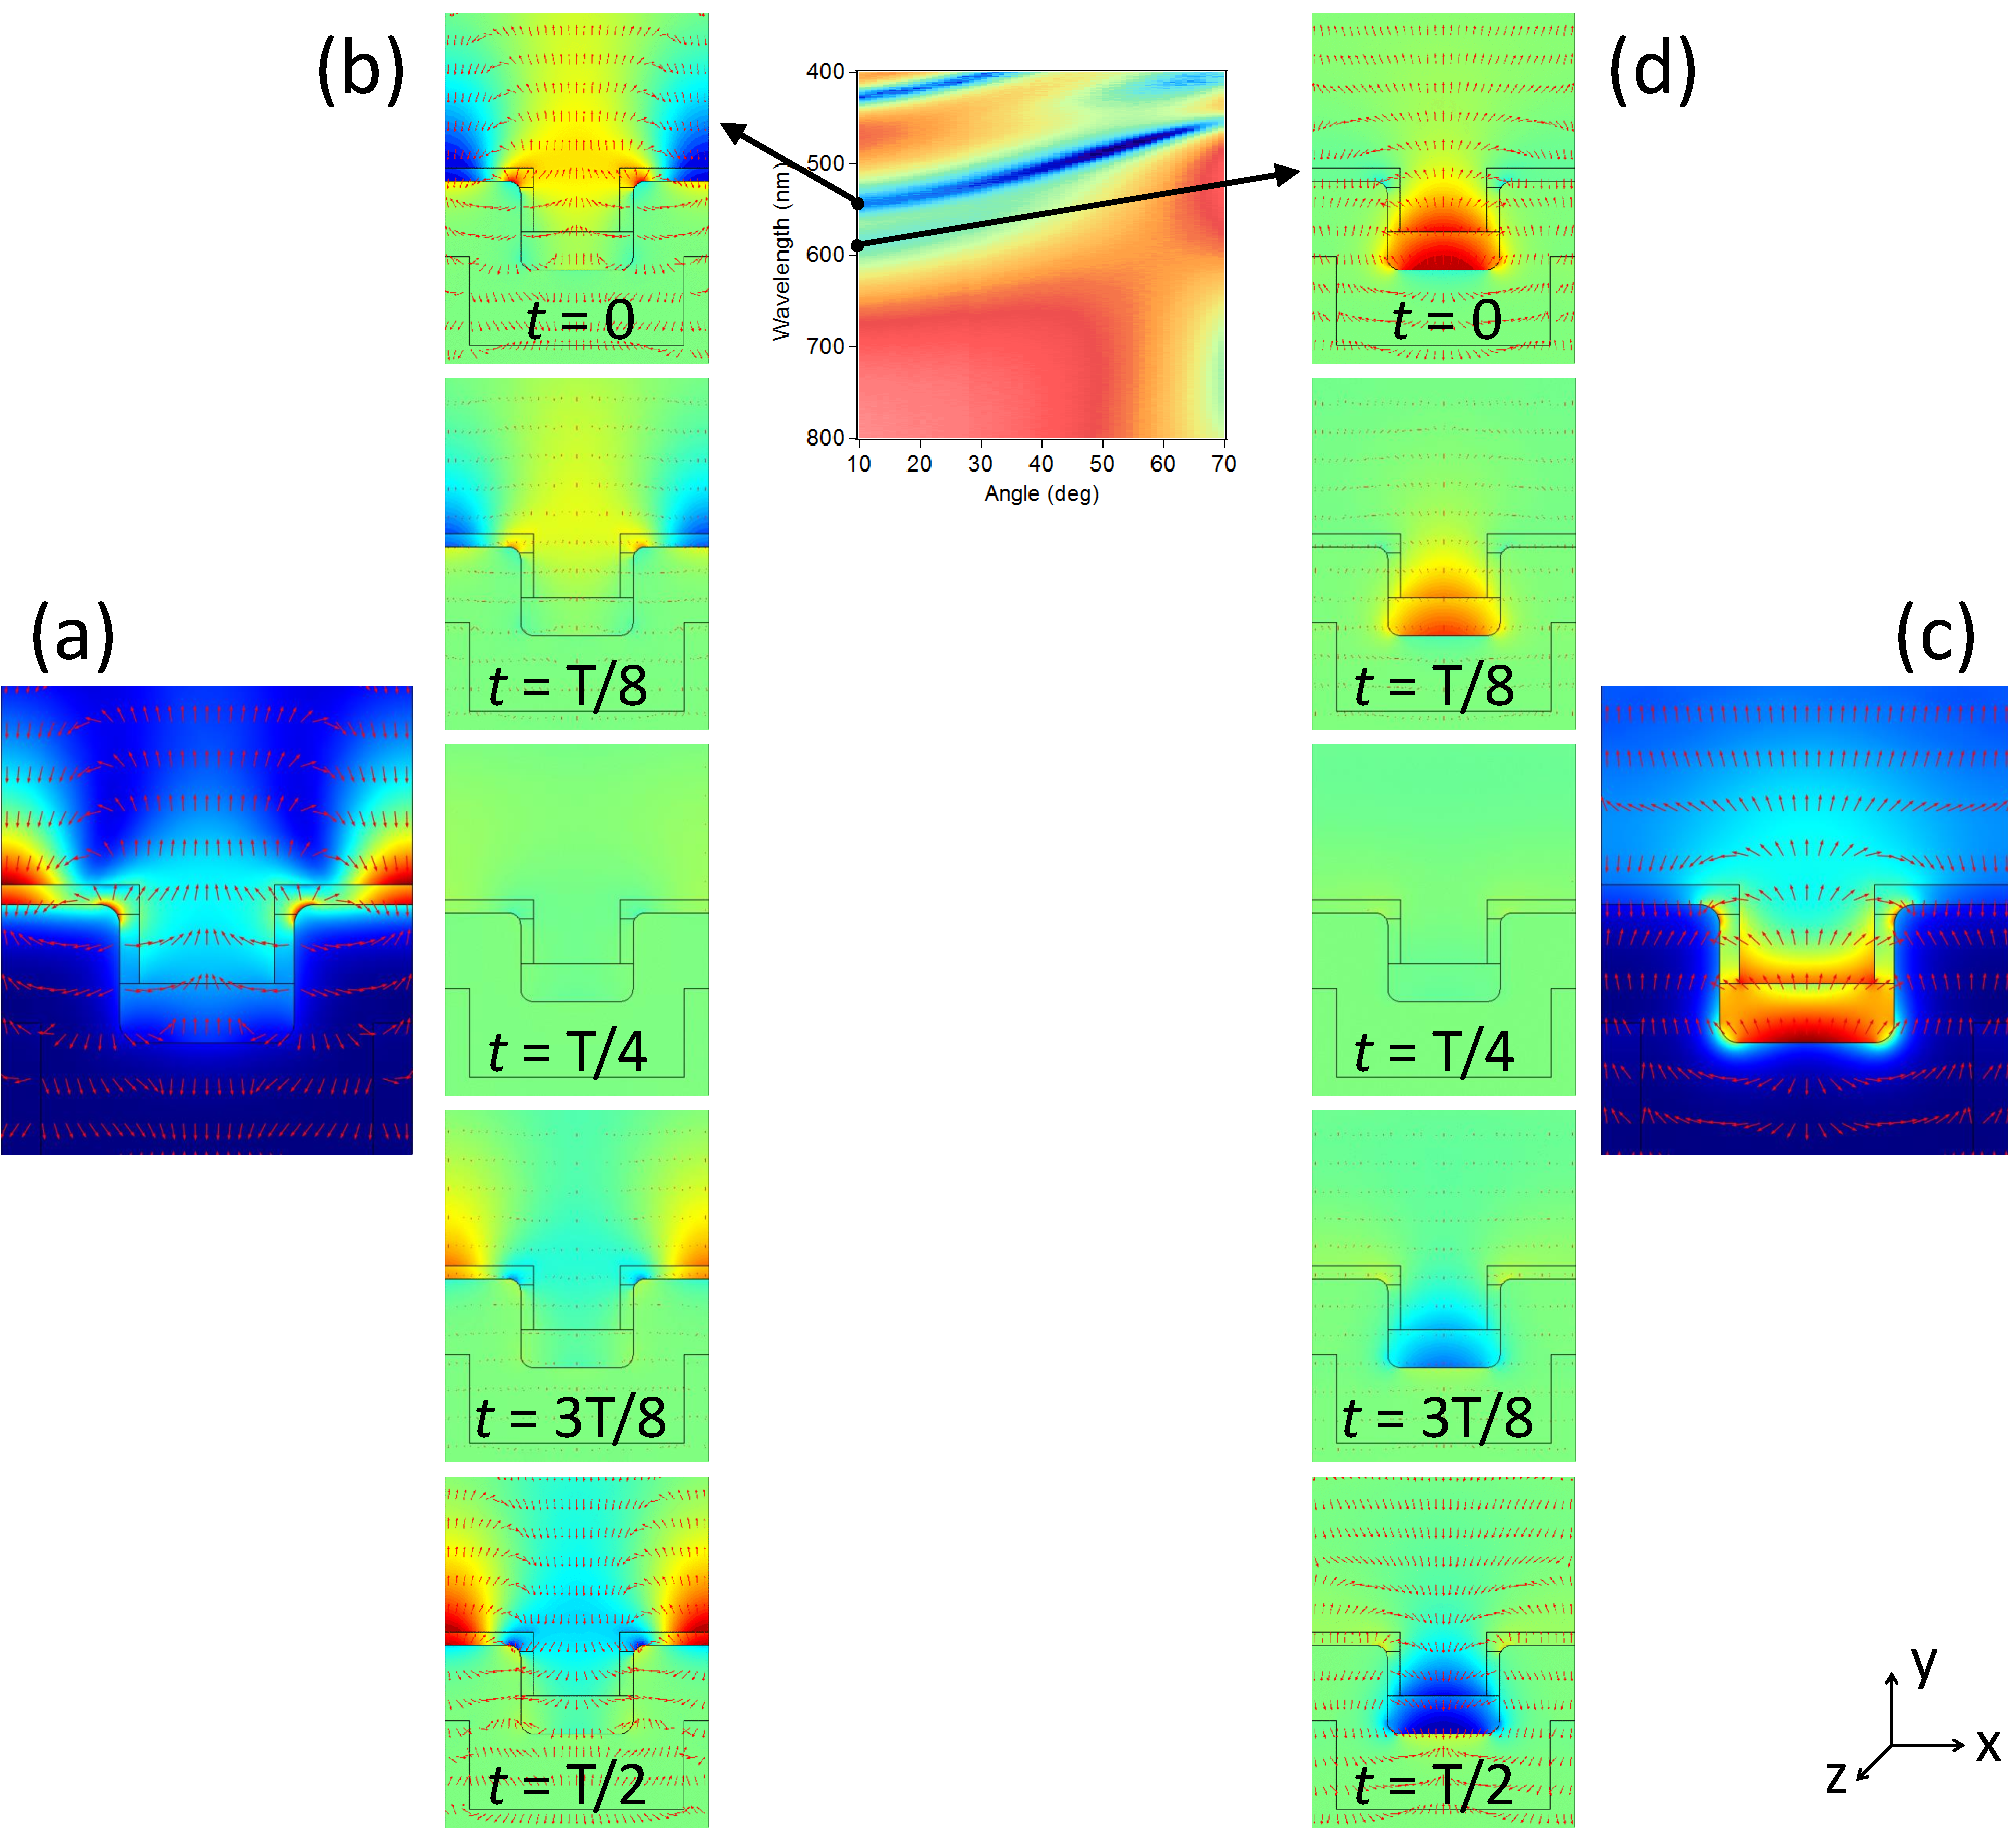
\includegraphics[width=\textwidth]{Fig12}
\caption{(a) Time averaged and (b) snapshots at time $t$ in the optical cycle T of $E_y$ nearfield intensity of the higher energy (plasmonic) mode at $\phi$=$0^{\circ}$ $\theta=0^{\circ}$. (c,d) same as above for the lower energy (waveguide) mode. The arrows on the diagrams indicate the Poynting vector (?). }
\label{7Fig12}
\end{figure}

Both SPP and waveguided modes are very sensitive to the dielectric environment as shown by Eqs.[grating,waveguide], and Fig.\,\ref{7Fig13} shows the change in these grating modes with increasing PS coverage. We can see both the narrower SPP resonances (black dashed lines) and broader waveguided modes (purple dashed lines) redshift with increasing PS coverage as expected. For the structure in Fig.\,\ref{7Fig13}(c) these two modes actually overlap, although no interaction occurs between them.
\begin{figure}[ht] 
\centering    
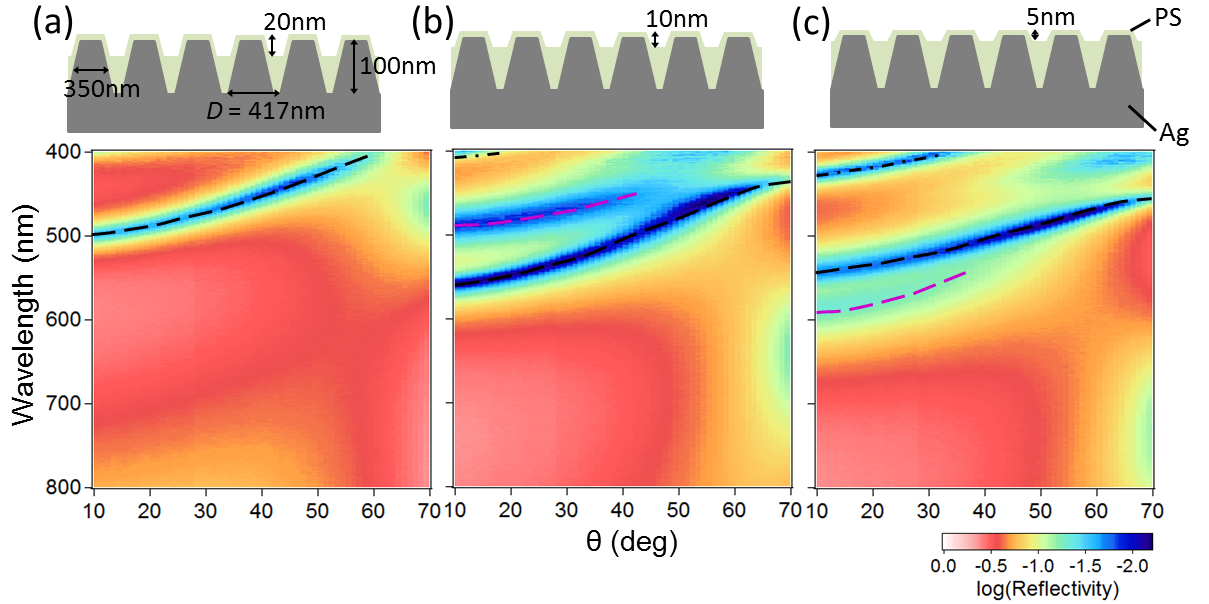
\includegraphics[width=\textwidth]{Fig13}
\caption{Schematic of PS-coated $D=417$\,nm Ag grating structure (above), and TM polarised reflectivity scans at $\phi=90^{\circ}$. Plasmonic modes are indicated by black lines, and waveguide modes by purple lines.}
\label{7Fig13}
\end{figure}

\subsection{CHPI-coated Ag gratings}
Fig.\,\ref{7Fig14} shows TM reflectivity scans for CHPI-coated Ag gratings with periodicities $D=556, 417, 278$\,nm at $\phi=0$ and $90^{\circ}$. The spectra for $D=556$ and 417\,nm are particularly similar, showing two exciton modes (red arrows), which strongly couple to the SPP grating mode (black) as the oscillations become resonant at $\phi=90^{\circ}$. Two excitons can also be observed for $D=278$\,nm, however the SPP mode is at a higher energy than for higher $D$ and thus the coupling occurs at $\phi=0^{\circ}$.
\begin{figure}[ht] 
\centering    
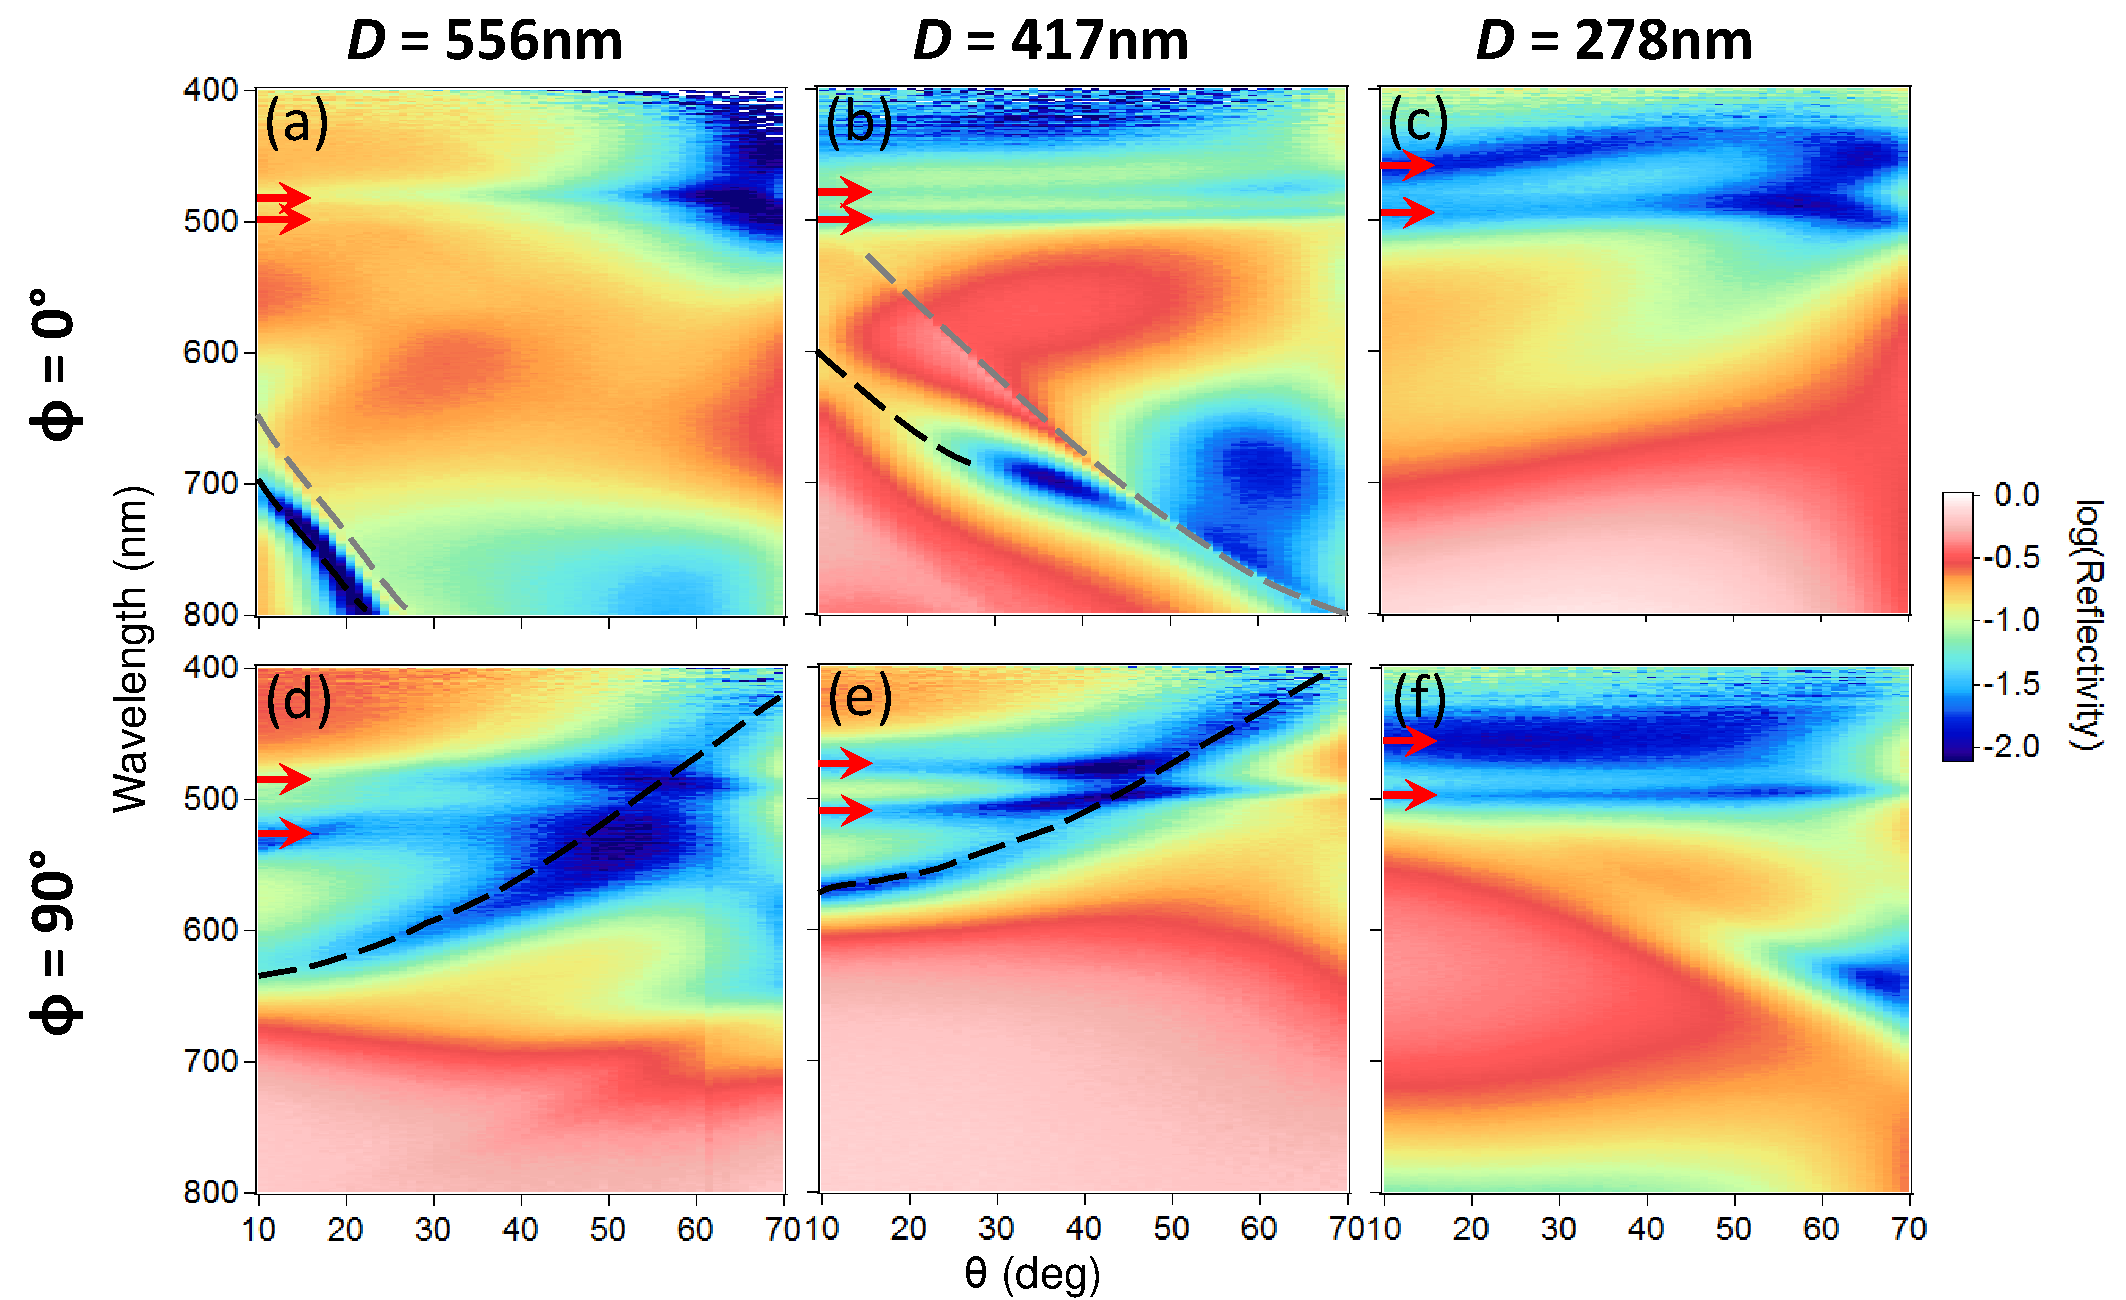
\includegraphics[width=\textwidth]{Fig14}
\caption{TM specular reflectivity scans of CHPI-coated Ag gratings with the labelled periodicity $D$ and at the labelled $\phi$. Photonic grating modes are marked by grey dashed lines, plasmonic grating modes are maked by black dashed lines, and excitons indicated by red arrows.}
\label{7Fig14}
\end{figure}

TM polarised reflectivity scans of a CHPI-coated Ag grating at $\phi=0^{\circ}$ [Fig.\,\ref{7Fig15}(a)] show two dispersionless exciton modes at 480 and 500\,nm (marked by arrows) far off resonance with grating modes. The persistent presence of a second exciton is only detected when SPPs can be excited, i.\,e.\,in TM polarisation [Fig.\,\ref{7Fig15}(a)] but not TE [Fig.\,\ref{7Fig15}(b)], nor in CHPI-coated planar Ag films [Fig.\,\ref{7Fig15}(c)]. It is also not observed for CHPI-coated non-plasmonic gratings, as seen in the CHPI-coated ETFE and Ti gratings. From Fig.\,\ref{7Fig15} we see that SPP excitation leads to the observation of an additional redshifted exciton with a splitting of 100\,meV. Its appearance only when SPPs are present rules out any influence from modified CHPI assembly in the grooves, which are in any case hundreds of times larger than the PbI layer spacing. We note slight changes in the CHPI coverage alter the positions and intensities of dispersive grating modes [{\it cf} Fig.\,\ref{7Fig17}(c), with a thinner CHPI coating], however the exciton modes remain essentially unchanged.

\begin{figure}[ht] 
\centering    
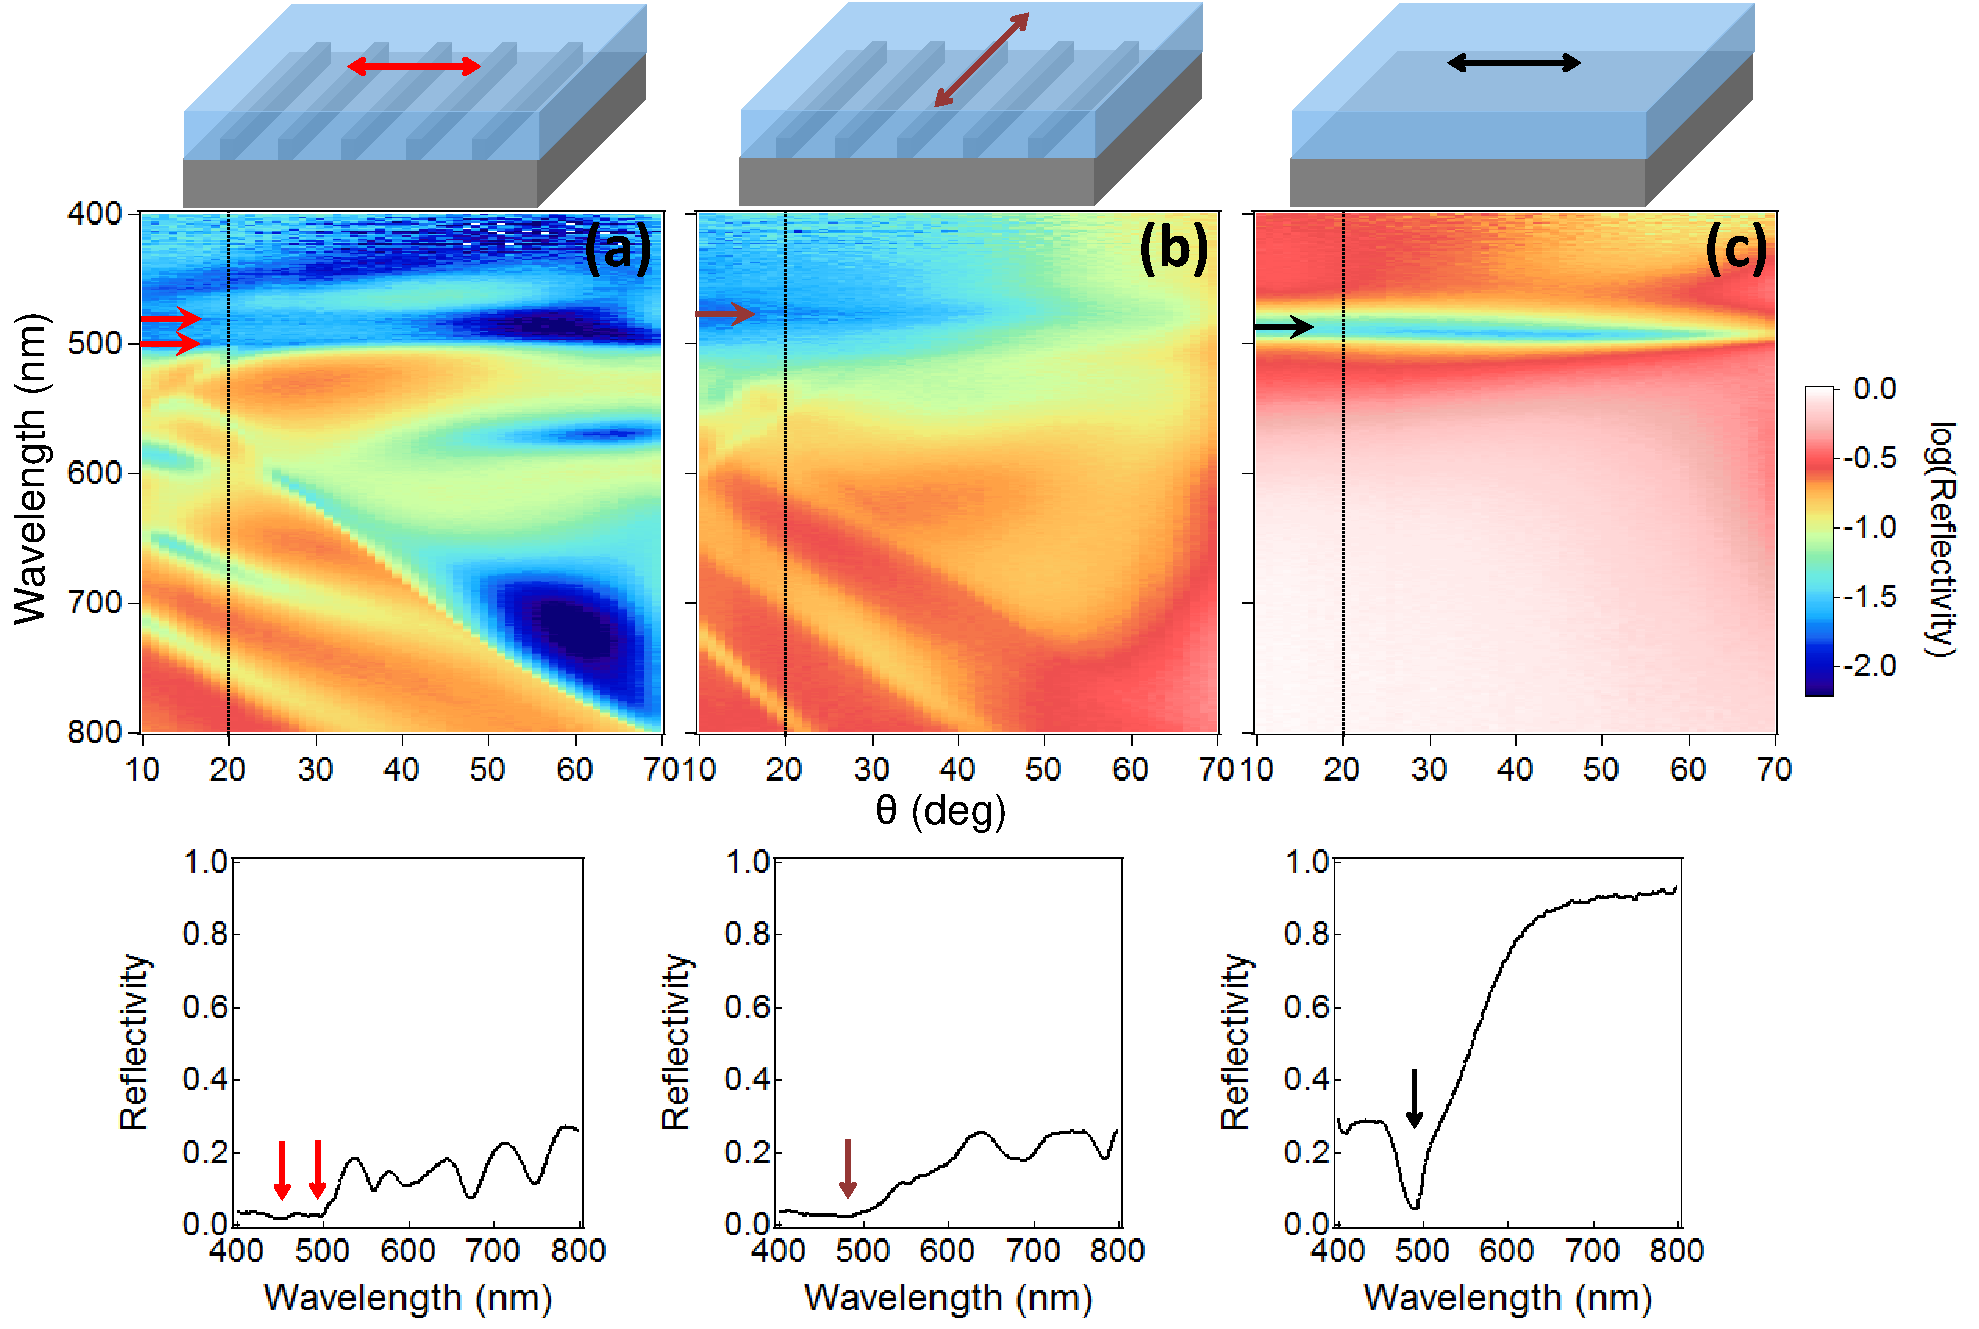
\includegraphics[width=\textwidth]{Fig15}
\caption{Specular reflectivity scans (above) at $\phi=0^{\circ}$: CHPI-coated Ag grating with (a) TM and (b) TE polarised light, and (c) CHPI-coated 120\,nm planar Ag film with TM polarised light; the reflectivity spectra at $\theta=20^{\circ}$ is shown below. The electric field orientation is shown above each scan, and positions of exciton modes indicated by arrows.}
\label{7Fig15}
\end{figure}

It is well known that the emitted energy of a dipole (exciton) is lowered when placed in front of a metallic surface due to interactions between the dipole and the reflected electromagnetic field \cite{Morawitz1969, Morawitz1974, Chance1974, Chance1975, Chance1975a, Ford1984}. Using the method of images, we can replace the metal and describe instead the coupling between an exciton in the CHPI ($\epsilon_1$) and its image exciton in the metal ($\epsilon_2$), modified by their respective dielectric environments. Chance \textit{et al.} \cite{Chance1975} showed the redshift in the emitted energy of an exciton ($\Delta E_{ex}$) oriented parallel to the interface can be approximated by
\begin{equation}
\centering
\Delta E_{ex} \sim \left( \frac{k_1}{l} \right) ^3 \text{Re} \left\{ \frac{\epsilon_2 - \epsilon_1}{\epsilon_2 + \epsilon_1} \right\} \Gamma_0 ,
\label{Redshift}
\end{equation}
where $l$ is the distance between the exciton and a metal surface, $k_1$ is the wavenumber of light in CHPI, and $\Gamma_0$ is the inverse exciton radiative lifetime without the metal. From this we can see the $l^{-3}$ dependence of the redshift as shown in Fig.\,\ref{fig2}(d), where the experimentally observed $\Delta E_{ex} \negmedspace \sim \negmedspace 100$\,meV corresponds to $l \negmedspace \sim \negmedspace 22$\,nm, close to the experimentally-determined CHPI thickness. Clearly $\Delta E_{ex}$ is also affected by the dielectric response of CHPI and Ag, and from Eq.\,\ref{Redshift} we see that $\Delta E_{ex}$ is maximised if $\epsilon_2 + \epsilon_1 \rightarrow 0$, i.\,e.\,when emission is resonant with an SPP on the metal-dielectric interface. 

The role of the SPP in this case is to outcouple the signal of the redshifted exciton. There are three main decay channels for dipole emission near a metal surface: direct emission to photons, emission to SPPs, and nonradiative processes such as the excitation of electron-hole pairs and lossy surface waves on the metal. Other nonradiative paths via defects or phonons are independent of $l$ and will be ignored in this analysis. Emission into SPPs provides an extra radiative decay channel as this signal can be extracted to the far field via the periodic nanostructure, and this mechanism has been used to improve the luminescence efficiency of light emitting devices \cite{Frischeisen2011, Kumar2012}. The relative decay probability for each process is calculated as a function of $l$ \cite{Ford1984} and shown in Fig.\,\ref{7Fig16}(a). Up to a CHPI thickness of 25\,nm, SPP mediated emission is the most important radiative decay channel with a maximum emission probability at 22\,nm, matching the experimentally observed $\Delta E_{ex}$. Even for thicker CHPI films we expect the exciton modes to remain at the same positions, because SPP emission becomes weak at large $l$ where $\Delta E_{ex}$ is negligible.

In our MQW perovskite system, localised excitons in periodically-spaced nearby QWs are optically coupled together to form collective exciton-polariton states an average distance $l$ from the Ag surface \cite{Pbbr2008, Baumberg1998, Kavokin1998, Vladimirova1998}. Therefore in CHPI-coated Ag gratings we observe both in-plane exciton-polaritons, and out-of-plane interactions that lead to `image-biexcitons', which are outcoupled via SPP emission with a binding energy of 100\,meV at room temperature [Fig.\,\ref{7Fig16}(b)]. For our grating system, the exciton and SPP modes become closer in energy with increasing $\phi$ [see below and Fig.\,\ref{7Fig17}(c)], and as a result splitting between the exciton modes (indicated by arrows in Fig.\,\ref{7Fig17}(c)) increases to around 185\,meV at $\phi=90^{\circ}$. The azimuthal dependence of the exciton splitting reflects the tuneable modification of the Coulomb interaction in this geometry, but however requires further theoretical development.
\begin{figure}[ht] 
\centering    
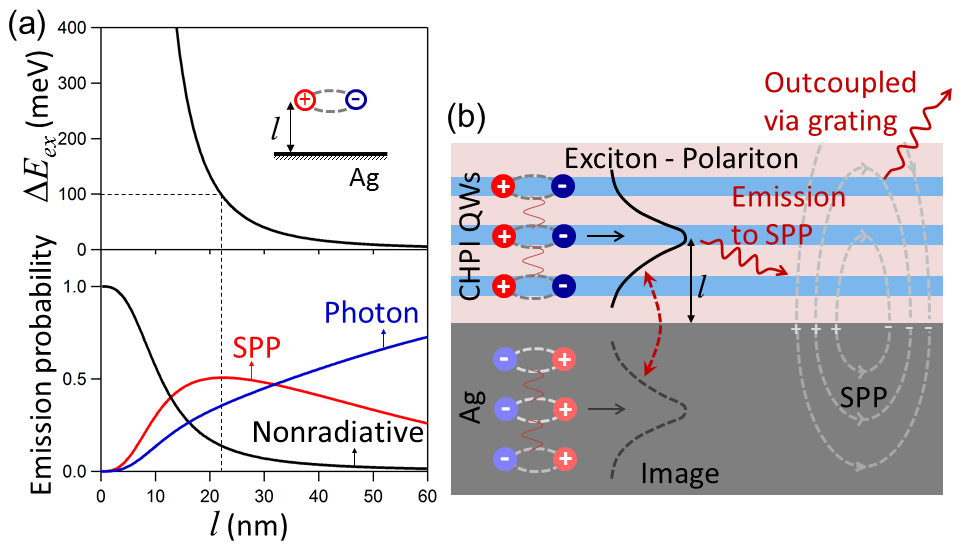
\includegraphics[width=0.8\textwidth]{Fig16}
\caption{(a) Change in emitted energy (top) and relative decay probabilities (bottom) of an exciton with energy 2.6\,eV placed distance $l$ from the Ag surface. The dashed line indicates the experimentally measured redshift. (b) Schematic mechanism for SPP-mediated emission of image-biexciton.}
\label{7Fig16}
\end{figure}

AFM image of the CHPI-coated Ag grating clearly shows the grating structure, although the CHPI coating is rather non-uniform [Fig.\,\ref{7Fig17}(a)]. Using AFM measurements, we find the CHPI forms a conformal coating around the Ag grating with thickness $\sim25$\,nm [Fig.\,\ref{7Fig17}(c)]. In TE polarisation, we only observe the presence of one exciton, without signature of any grating modes, similar to the CHPI-coated Ti gratings. In TM polarised reflectivity scans, as well as strong excitnos (red arrows) we also observe $m=\pm1$ photonic and plasmonic grating modes [Fig.\,\ref{7Fig17}(c)].  As the SPP modes become resonant with the exciton and image exciton, the light-matter modes strongly couple and produce an anticrossing in the reflectivity of 0.25\,eV. Extracting the mode positions from the $\phi=90^{\circ}$ scan [Fig.\,\ref{fig3}(d)] allows them to be fit to a three oscillator model using the Hamiltonian
\begin{equation}
\centering 
\hat{H}=\left( \begin{matrix} 
E_{ex} & 0 & \Omega_{ex}/2 \\
0 & E_{bx} & \Omega_{bx}/2 \\
\Omega_{ex}/2 & \Omega_{bx}/2 & E_{pl} 
\end{matrix} \right) ,
\end{equation}
where $E_{ex}$, $E_{bx}$ and $E_{pl}$ are the energies of the exciton-polariton, image-biexciton and plasmonic grating modes respectively, while $\Omega_{ex}$ and $\Omega_{bx}$ represent the interaction between the SPP and exciton/image-biexciton. From this we find Rabi splittings of $\Omega_{ex}=150$\,meV and $\Omega_{bx}=125$\,meV. 
These are greatly enhanced because of the large confinement of the plasmonic optical field in the thin PbI QW layers. The Rabi splitting is given by $\Omega \propto \sqrt{f_{osc} N_{QW}/V}$, where the oscillator strength ($f_{osc}$) of the CHPI is assumed to be similar for coupling to photons or plasmons, the number of QWs ($N_{QW}$) is proportional to the CHPI thickness, and the mode volume ($V$) is here proportional to the optical mode size. Comparing to Fabry-Perot planar CHPI microcavities in strong coupling \cite{Pradeesh2009b} which have CHPI thickness of 72\,nm, cavity length of 407\,nm, and a Rabi frequency of $\Omega_{FP}=65$\,meV, the simple scaling above predicts $\Omega_{SPP} \sim \Omega_{FP} \sqrt{(22/72).(407/22)}$=156\,meV, in excellent agreement with our measurements. Using SPPs to strongly couple to the excitons thus dramatically reduces the cavity length, thus enhancing the light-matter coupling.

\begin{figure}[ht] 
\centering    
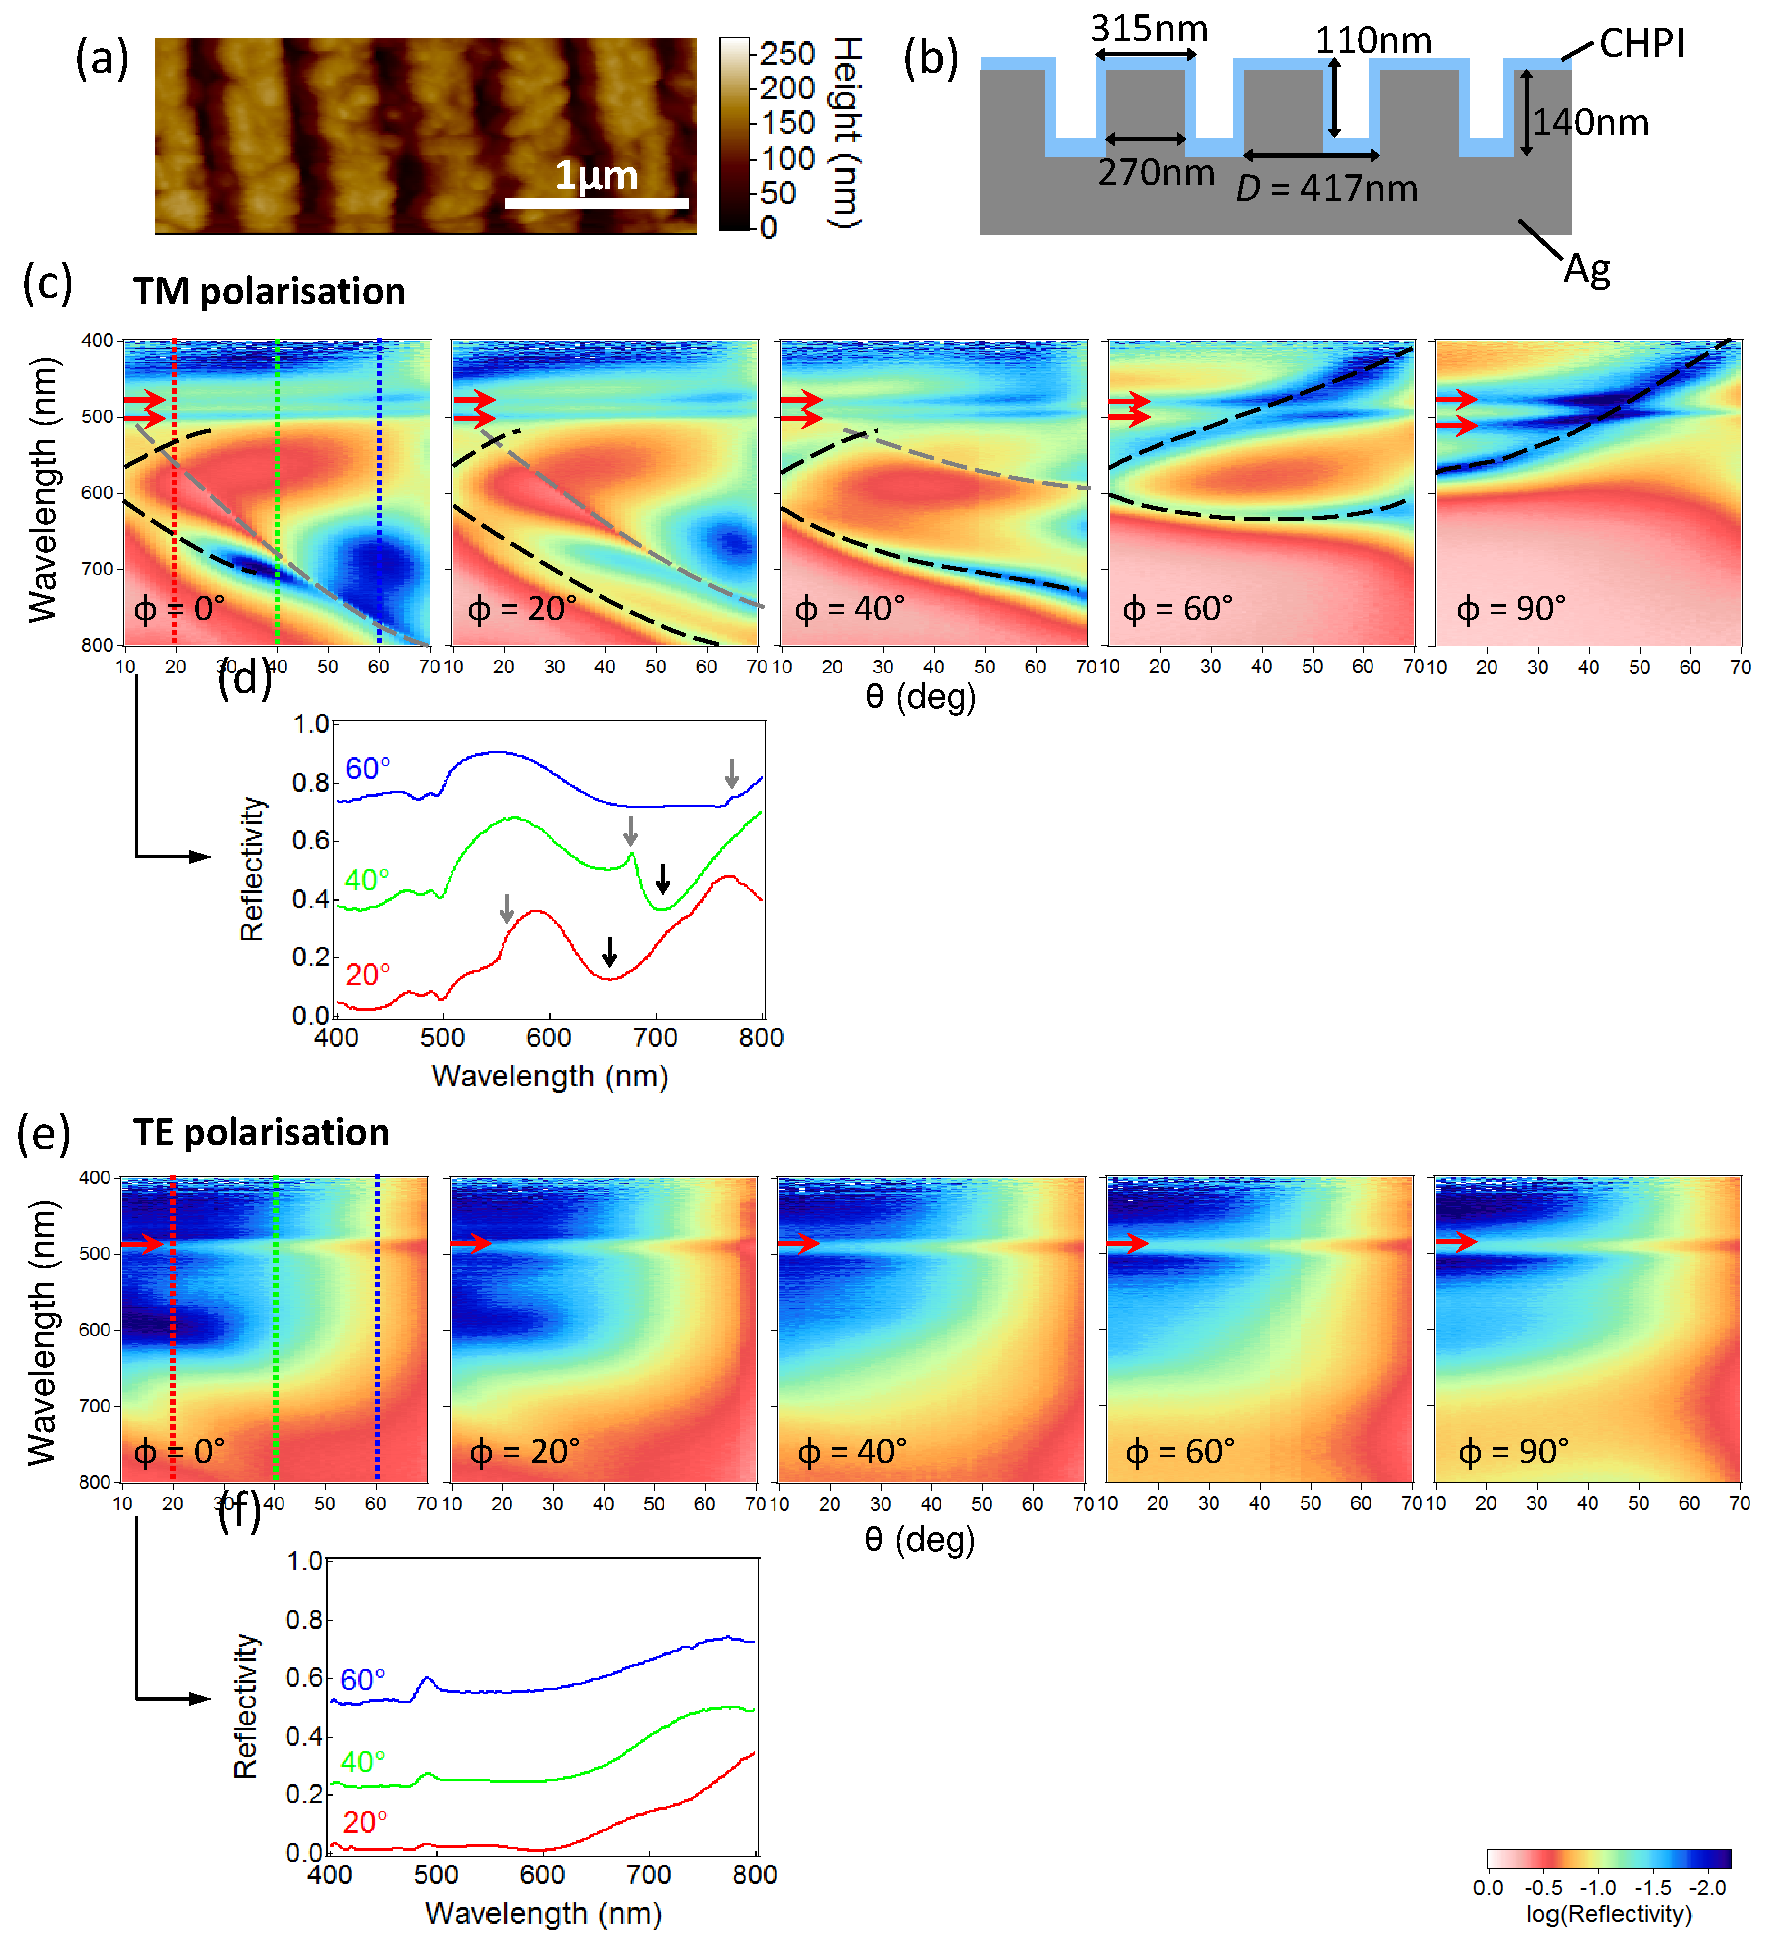
\includegraphics[width=\textwidth]{Fig17}
\caption{(a) AFM image and (b) schematic of CHPI-coated Ag grating structure. (c) TM polarised reflectivity scans of $D=417$\,nm Ag grating at labelled $\phi$, and (d) reflectivity spectra at indicated $\theta$ value for $\phi=0^{\circ}$. (e,f) Same as above for TE polarisation. Photonic grating modes are indicated by grey lines/arrows on reflectivity scans/spectra respectively, plasmonic gratings modes by black lines/arrows, and excitons by red arrows.}
\label{7Fig17}
\end{figure}

We calculate the full eigenstates of the system using FEM simulations. These confirm the anticrossings observed, and provide the optical field profiles.
In the case of strong coupling at $\phi=90^{\circ}$, the time-averaged near-field shows strongest intensity inside the CHPI which coats the bottom surface of the grating, with a rapid evanescent decay away from the interface [Figs.\,\ref{fig4}(b,c)]. The mode is thus both laterally confined by the grating as well as being trapped inside the surface layers where it couples to the excitons.

The SPP $E$-field direction is primarily perpendicular to the metal-dielectric interface, while excitons in CHPI QWs are polarised parallel to this interface \cite{Pradeesh2009b, Mitzi2001b}.  Simulated $\phi=90^{\circ}$ spectra for in- and out-of-plane exciton dipoles are shown in Figs.\,\ref{fig4}(d,e) respectively. While strong coupling is seen for both dipole orientations, the bare exciton is only seen for the in-plane dipole. It thus appears that the coupling between the excitons and their images are responsible for mixing the dipole orientations, enabling the strong coupling with the SPP mode. The polariton states mix excitons within the perovskite which are delocalised across many PbI monolayers, with SPPs which are tightly confined to the CHPI layer above the Ag grating and laterally localised in the grating slits by the coupling of standing waves. Such light-matter polaritonic quasiparticles thus combine organic, inorganic and plasmonic components in an unusual fashion.
\begin{figure}[ht] 
\centering    
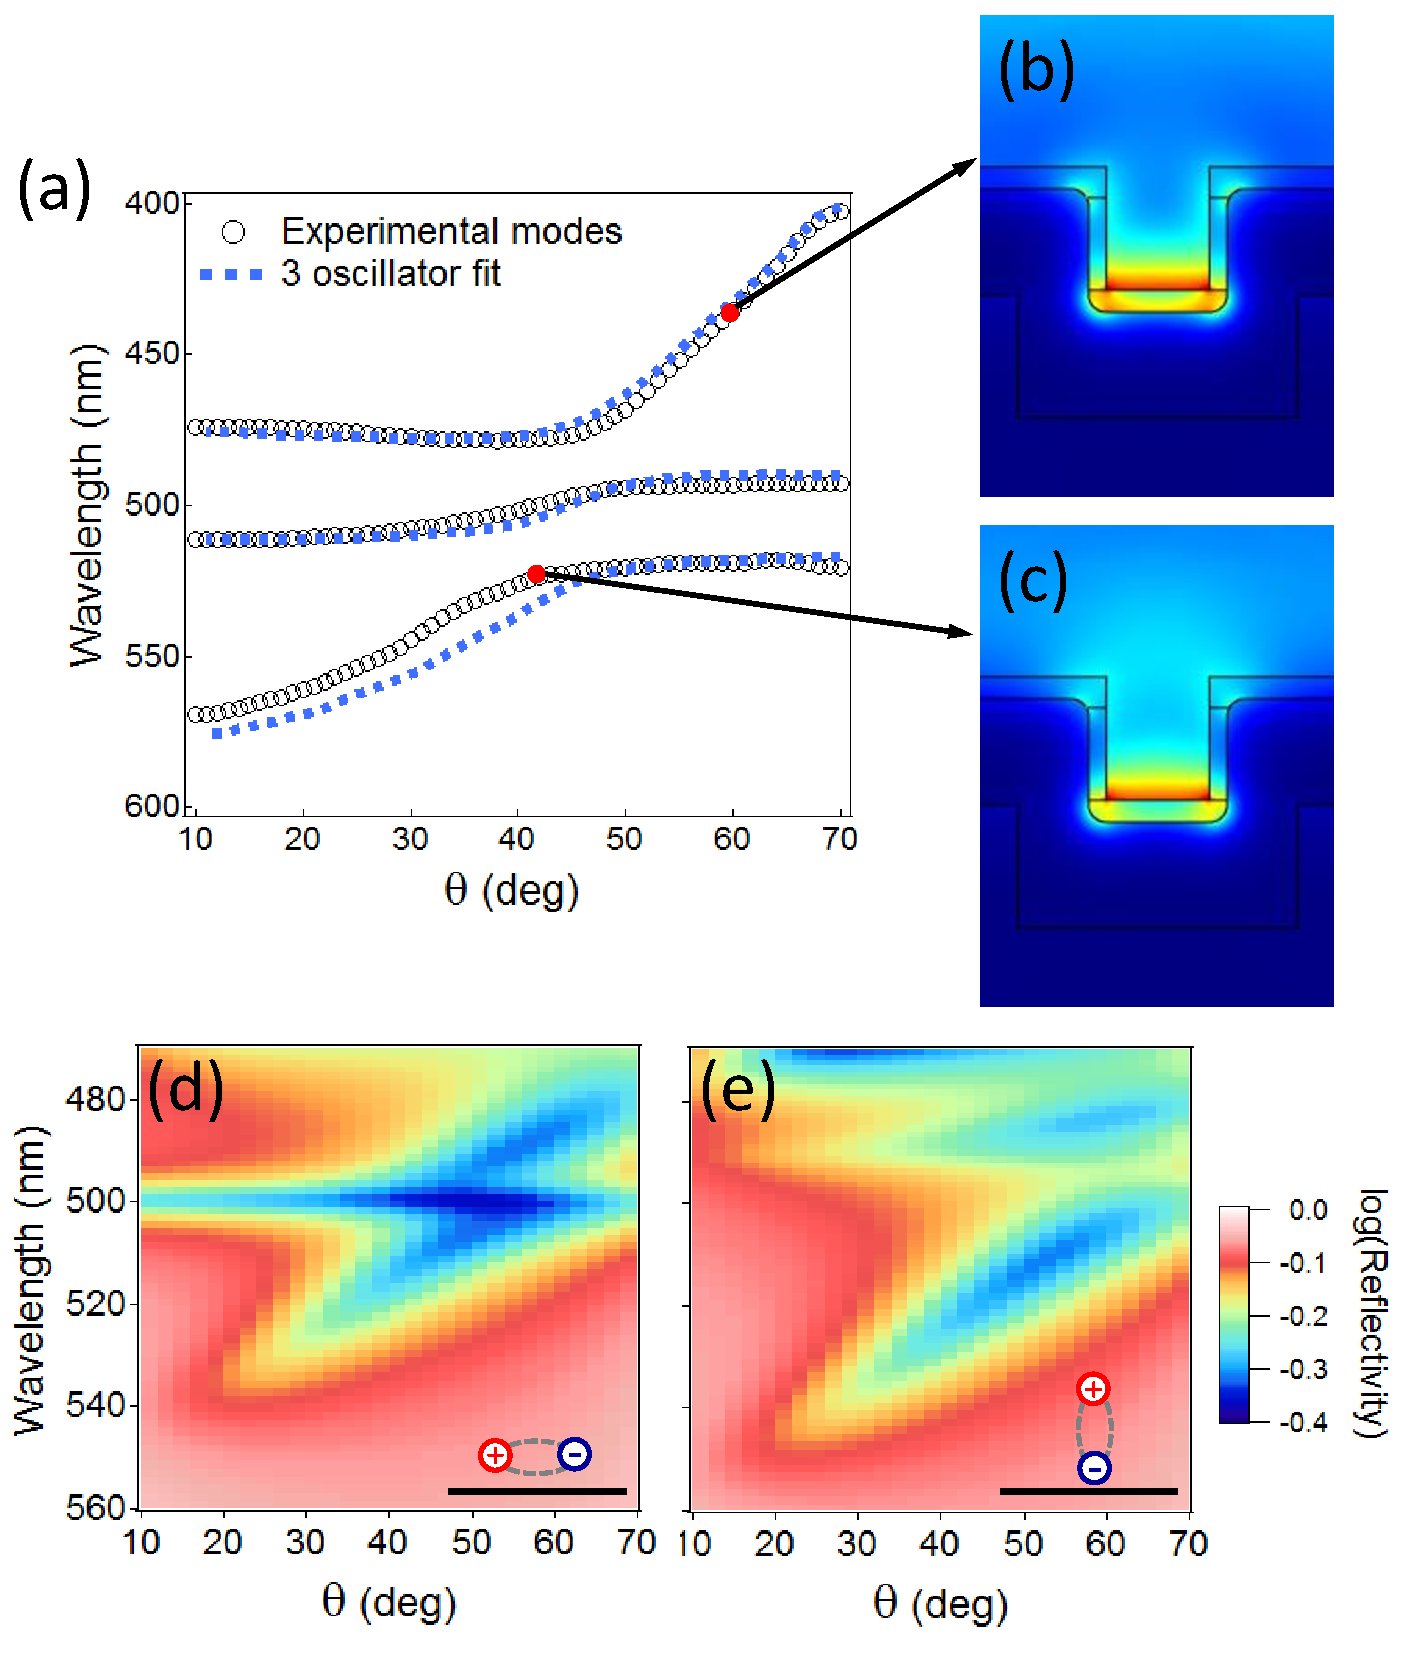
\includegraphics[width=0.8\textwidth]{Fig18}
\caption{(a) Extracted spectral mode positions for $\phi=90^{\circ}$ reflection dips (open circles), and fit from three oscillator coupling model (dashed lines). (b,c) Time-averaged $E$-field intensity profiles ($\vec{E}\cdot\vec{E}$) as indicated. (d,e) Simulated reflection spectra for (d) in-plane and (e) out-of-plane exciton dipoles.}
\label{7Fig18}
\end{figure}

\section{Conclusions}
A simple 1D plasmonic periodic structure can give host to a wide range of grating modes: photonic modes due to the interference of light, excitement of SPPs on the surface of the metal, or laterally localised modes such as channel plasmons or waveguide modes. The positions and efficiencies of many of these modes depends sensitively on the geometry of the grating and the dielectric environment provided by any overcoating materials. Thus it is not always easy to predict what can be observed in optical spectra.

In CHPI-coated Ag gratings, we observe evidence of image-biexcitons with binding energy 100\,meV at room temperature. Such quasiparticles arise from the interaction between excitons and their images in the metal, and are outcoupled from the grating structure via SPP emission. These out-of-plane biexciton states mediate coupling between in-plane QW excitons and out-of-plane SPP grating modes. This enables the observation of strong coupling at room temperature with Rabi splittings of 150 and 125\,meV for the exciton and image-biexciton respectively. Both the biexciton binding energy and strong coupling Rabi splitting is tuneable by small changes in the structure of the coated gratings.

Strong coupling has previously been observed between inorganic or organic excitons and Au nanoslit gratings at low temperature. The coupling constants in these systems are much smaller compared to CHPI at room temperature: 55\,meV for 50\,nm J-aggregate films at 77\,K \cite{Vasa2010}, and 8\,meV for 10\,nm GaAs QWs at 10\,K \cite{Vasa2008}. One key difference is that for the III-V semiconductors the QWs have to be spaced at least 20\,nm from the metal surface to maintain their optical quality. In contrast our 25\,nm thick CHPI film is prepared directly on the metal, and still gives strongly radiative exciton modes because the organic sandwich protects the PbI QW layers. Theoretically Fig.\,\ref{fig2}(d) shows that excitons remain radiative via SPP coupling for film thickness above 10\,nm. Hence the perovskite system is well suited to manipulate light-matter interactions. Such modification of the exciton and SPP states is of great interest for future optoelectronic devices, involving ultrathin semiconductors including the layered van der Waals materials based on graphene and dichalcogenides.